\documentclass[12pt]{report}

\usepackage{setspace}
\usepackage{bibcontents}
\usepackage{times,amsmath,epsfig}
\usepackage[T1]{fontenc}
\usepackage{epstopdf}
\usepackage{latexsym}
\usepackage{algorithm}
\usepackage{algorithmic}
\usepackage{epsfig}
\usepackage{amssymb}
\usepackage{amsfonts}
\usepackage{graphicx}
\usepackage{bm}
\usepackage{balance}
\usepackage[labelformat=simple]{subcaption}
\usepackage{titlesec} % used for additional level 
\usepackage{array} % used for scaling table 

\setlength{\textheight}{8.63in}
\setlength{\textwidth}{5.9in}
\setlength{\topmargin}{-0.2in}
\setlength{\oddsidemargin}{0.3in}
\setlength{\evensidemargin}{0.3in}
\setlength{\headsep}{0.0in}
\linespread{1.25}
\newcommand{\ie}[0]{\textit{i.e.}}
\newcommand{\eg}[0]{\textit{e.g.}}
\newcommand{\etal}[0]{\textit{et al.}}

\newcommand{\keobf}{\textit{$(k,\epsilon)$-obf}}
\newcommand{\argmin}{\operatornamewithlimits{argmin}}
\newcommand{\norm}[1]{\left\lVert#1\right\rVert}
\newcommand{\repAn}[0]{\textnormal{Rep-An}}
\newcommand{\augcrr}[0]{\textnormal{AUG-CRR}}
\newcommand{\augrr}[0]{\textnormal{AUG-RR}}
\newcommand{\augc}[0]{\textnormal{AUG-C}}
\newcommand{\aug}[0]{\textnormal{AUG}} 
\newcommand{\funcname}[0]{\textit{GenAnonymization}}

\renewcommand\thesubfigure{(\alph{subfigure})} % for
\newtheorem{theorem}{Theorem} 
\newtheorem{definition}{Definition}
\newtheorem{problem}{Problem}
\newtheorem{example}{Example}
\newtheorem{lemma}{Lemma}
\newtheorem{proof}{Proof}
\newcolumntype{L}[1]{>{\raggedright\let\newline\\\arraybackslash\hspace{0pt}}m{#1}}


\begin{document}
\setcounter{secnumdepth}{2}

% \newcommand{\brk}{\vspace*{0.15in}}
% \newcommand{\ssp}{\singlespacing}
% \newcommand{\dsp}{\doublespacing}
% \newcommand{\hbrk}{\\[0.4in]}
\newcommand{\bi}{\begin{itemize}}
\newcommand{\ei}{\end{itemize}}
\newcommand{\be}{\begin{enumerate}}
\newcommand{\ee}{\end{enumerate}}
\newcommand{\bd}{\begin{description}}
\newcommand{\ed}{\end{description}}
\newcommand{\vj}{\vspace{-1em}}
\newcommand{\svj}{\vspace{-0em}}


% \titleformat{\paragraph}
% {\normalfont\normalsize\bfseries}{\theparagraph}{1em}{}
% \titlespacing*{\paragraph}
% {0pt}{3.25ex plus 1ex minus .2ex}{1.5ex plus .2ex}

%\renewcommand{\baselinestretch}{1}  %turns on double spacing
%
%\doublespacing
% No page number on the title page
\thispagestyle{empty}

% Center the title
%\begin{center}


\title{Towards Graph Analytic and Privacy Protection}
\author{\large Dongqing Xiao}
%\date{Draft. \today}
\date{\Large A Proposal for a PhD Dissertation in Computer Science\\[1cm]
\large Worcester Polytechnic Institute, Worcester, MA\\[5mm]
Dec 2016
\vfill
\begin{minipage}{18cm}
\textbf{Committee Members:}\\
Dr. Mohamed Y. Eltabakh, Assistant Professor, Worcester Polytechnic Institute. Advisor.\\
Dr. Elke A. Rundensteiner, Professor, Worcester Polytechnic Institute.\\
Dr. Xiangnan Kong, Assistant Professor, Worcester Polytechnic Institute.\\
Dr. Yuanyuan Tian, Researcher, IBM Almaden, External member.
\end{minipage}
}

\maketitle


% end of titlepage
\newpage

% This is the command for doublespacing when you use the setspace
% package
% Please do NOT use \baselinestretch, this will mess up everything,
% cause earthquakes, tornados and lots of questions for me...
% If you need a singlespaced paragraph (BAD STYLE!!!), use
% \singlespacing or \onehalfspacing and enclose it together with the
% paragraph in braces {\singlespacing This is my text... blah blah blah}
%
%\doublespacing

% Now you can start to be creative.
% First, you need an abstract.
% Fortunately, LaTeX has thought of that, so it's very easy:
%
\begin{abstract}
In the real world, graph structured data is ubiquitous. For instance, social networks, communication networks, biological networks, etc. can all be modeled as graphs. Various graph analysis mining methods have been proposed to deepen the understanding of the graph data, in particular in sequential platforms. However, the graph size continues to increase and becomes massive involving billions of vertices and edges. Such massive graphs can easily exceed the available memory of a single commodity computer and pose a new challenge for graph mining tasks.
One of the methods to deal with large graphs is to exploit parallel programming paradigms including MapReduce. 
Within this scope, we study how to design an efficient distributed triangle listing algorithm for web-scale graphs with MapReduce. 

\textit{$\bullet$~Distributed triangle listing algorithm} Inspired by the theoretical and practical significance, the triangle listing problem has then been studied in MapReduce.  Triangle listing requires accessing the neighbors of the neighbor of a vertex, which may appear arbitrarily in different graph partitions (poor locality in data access).  Existing algorithms suffer from generating and shuffling huge amounts of intermediate data, where interestingly, a large percentage of this data is redundant. Inspired by this observation, we present the {\em ``Bermuda''} method that effectively reduces the size of the intermediate data via redundancy elimination and sharing of messages whenever possible. 

Besides, in many real-world applications, graphs are not deterministic but probabilistic in nature for a variety of reasons. In these cases, data is represented as an uncertain graph whose edges are accompanied with a probability of existence. Uncertain graphs have been shown to be invaluable dataset for a variety of real applications and analytic tasks.  
However, the raw uncertain graph is particularly sensitive: it contains personal details and  sensitive connections between them which are not public and should not be revealed. Thus, before such uncertain graphs can be released for research purposes, the data needs to be anonymized to prevent potential re-identification attacks. However, previous graph anonymization approaches are all geared towards deterministic graphs. It calls for novel anonymization techniques that are able to cope with the additional uncertainty explicitly.  Within this scope, we study uncertain graph anonymization techniques for resisting privacy attacks depend on the node degree statistic and  degree probabilistic distribution. 

\textit{$\bullet$~Degree Anonymization over Uncertain Graphs} In this work, we consider that the adversary relies upon the knowledge of node  degree statistic (the expected value) in devising a matching attack for nodes in the released uncertain graph, which is a well-known privacy attack while in the new context--uncertain graph. However, applying existing methods straightforward can not provide efficient privacy protection meanwhile incurring a large amount of utility loss. To prevent such matching attack, we consider {\keobf}, a popular privacy notation, to protect such degree-based matching attack. We extend the existing {\keobf}framework to work over the uncertain graph. We also design a set of heuristic-based techniques to make the anonymization mechanism efficient meanwhile preserving data utilities, especially the graph reliability. Extensive experiments on large real datasets show the satisfactory performance of our methods in terms of privacy protection, efficiency, and practical utilities. 

\textit{$\bullet$~Probabilistic Degree Anonymization over Uncertain Graphs} In this work, we consider that the adversary relies upon the knowledge of node  degree probability distribution rather than aggregated statistic in devising a matching attack for nodes in the released uncertain graph. We formally present the definition of probabilistic degree-based node re-identification attack, which is a newly identified privacy attack in the uncertain graph. Similarly, we extend the concept of {\keobf} to protect such matching attack. We develop a general framework which injects uncertainty to edges in the uncertain graph for obtaining {\keobf}. In particular, we propose to utilize the clustering result of probabilistic degree for guiding the perturbation which maximizes the likelihood of providing higher privacy guarantee. We also consider utilizing the genetic algorithm for the optimization of edge perturbation strategy. Extensive studies including privacy protection, efficiency, and practical utility evaluation will be conducted on large real datasets to evaluate the effectiveness and efficiency of my proposed approaches. 
\end{abstract}

% From here on, we need Roman page numbers according to the library
% regulations. So let's assign those.

\pagenumbering{roman} % or {Roman} if you like them capitalized

% The next thing is the Preface (``Acknowledgements'').
% No standard environment for that, so we'll format it by hand.
%

\clearpage




\tableofcontents

% THAT'S IT. REALLY. Everything else is automatic. No formatting, no headline.
% All predefined.
% Now - just as easy - the List of Figures.
% This will catch all objects enclosed in \begin{figure}\end{figure}
% statements.

%\listoffigures

% There is also a list of tables, if you have any.
% This will catch all objects enclosed in \begin{table}\end{table}
% statements.
%\listoftables


% And we need a clear separation between preface and text, otherwise
% the numbering gets confused.

\clearpage

\pagenumbering{arabic}
\setcounter{page}{1}
\newpage
\noindent
\noindent
\begin{center}
{\large \bf Acknowledgments}
\end{center}

\noindent
\noindent

I express my sincere thanks to my advisor Prof. Mohamed Eltabakh. My thank you goes to the members of my Ph.D. committee, Prof. Elke Rundensteiner, Prof. Xiangnan Kong and Dr. Yuanyuan Tian. My thank you also goes to all other previous and current DSRG members for their useful discussion and feedback. 
\chapter{Introduction}
\label{chp:introduction}

\section{Motivation}
\label{sec:motivation}

Network data has become increasingly important in recent years of the greater importance of various application domains such as Web, social network, biological networks, and communication networks. The semantics and the interpretation of the nodes and the links may vary with application domain, {\eg}, in a social network node can represent individuals and their connection captures friendship, while in a protein-to-protein network (PPI) nodes are proteins and connections refer to their interactions. These graph data carries valuable information and are analyzed in various ways to exact knowledge. For example, social networks provide significant insight about psychological behavior of individuals or PPI network are widely stuided to eclucidate mechasim of diseases. 

Before such graph data can be released for XX . 

\section{State-Of-the-Art}
\label{sec:state-of-the-art}
\subsection{Distributed Triangle Listing Algorithms}
Triangle listing is a basic operation of the graph analysis. Many research works have been conducted on this problem, which can be classified into three categories: in-memory algorithms, external-memory algorithms and distributed algorithms. Here, we briefly review these works. 

\textbf{In-Memory Algorithm.} 
The majority of previously introduced triangle listing algorithms are the In-Memory processing approaches. Traditionally, they can be further classified as Node-Iterator\cite{Alon_Yuster_Zwick_1997,Batagelj_Mrvar_2001,Schank_2007} and Edge-Iterator ones\cite{
Itai_Rodeh_1978,Chiba_Nishizeki_1985} with the respect to iterator-type. Authors \cite{Itai_Rodeh_1978,Chiba_Nishizeki_1985,Schank_2007}improved the performance of in-memory algorithms by adopting degree-based ordering. 
Matrix multiplication is used to count triangles \cite{Alon_Yuster_Zwick_1997}. However, all these algorithms are inapplicable to massive graphs which do not fit in memory. 

\textbf{External-Memory Algorithms.} In order to handle the massive graph, several external-memory approaches were introduced \cite{H14,Kim_Han_Lee_Park_Yu_2014,GraphChi}. Common idea of these methods is: (1)~Partition the input graph to make each partition fit into main-memory, (2)~Load each partition individually into main-memory and identify all its triangles, and then remove edges which participated in the identified triangle, and (3)~After the whole graph is loaded into memory buffer once, the remaining edges are merged, then repeat former steps until no edges remain. These Algorithms require a lot of disk I/Os to perform the reading and writing of the edges. 
Authors ~\cite{H14,Kim_Han_Lee_Park_Yu_2014} improved the performance by reducing the amount of disk I/Os and exploiting multi-core parallelism. External-Memory Algorithms show great performance in time and space. However, the parallelization of external-memory algorithms is limited. External-memory approaches cannot easily scale up in terms of computing resources and parallelization degree.

\textbf{Distributed Algorithms.} 
Another promising approach to handle triangle listing on large-scale graphs is the distributed computing. Suri {\etal} \cite{Suri_Vassilvitskii_2011} introduced two Map-Reduce adaptions of NodeIterator algorithm and the well-known Graph Partitioning (GP) algorithm to count triangles. The Graph Partitioning algorithm utilizes one universal hash partition function over nodes to distribute edges into overlapped graph partitions, then identifies triangles over all the partitions. Park {\etal} \cite{parkmapreduce2014} further generalized Graph Partitioning algorithm into multiple rounds, significantly increasing the size of the graphs that can be handled on a given system. The authors compare their algorithm with GP algorithm \cite{Suri_Vassilvitskii_2011} across various massive graphs then show that they get speedups ranging from 2 to 5. In this work, we show such large or even larger speedup (from 5 to 10) can also be obtained by reducing the size intermediate result directly via our methods. Teixeira {\etal} \cite{Teixeira_2015} presented Arabesque, one distributed data processing platform for implementing subgraph mining algorithms on the basis of MapReduce framework.  Arabesque automates the process of exploring a very large number of subgraphs, including triangles. However, these MapReduce algorithms must generate a large amount of intermediate data that travel over the network during the shuffle operation, which degrade their performance. Arifuzzaman {\etal} \cite{Patric} introduced an efficient MPI-based distributed memory parallel algorithm (Patric) on the basis of NodeIterator algorithm. The Patric algorithm introduced degree-based sorting preprocessing step for efficient set intersection operation to speed up execution. 
Furthermore, several distributed solutions designed for subgraph mining on large graph were also proposed \cite{Pregel,Shao_2014}. Shao {\etal} introduced the PSgl framework  to iteratively enumerate subgraph instance. Different from other parallel approaches, the PSgl framework completes relies on the graph traversal and avoids the explicit join operation. These distributed memory parallel algorithms achieve impressive performance over large-scale graph mining tasks. These methods distributed the data graph among the worker's memory, thus they are not suitable for processing large-scale graph with small clusters.

\subsection{Graph Anonymization}
Uncertain graph anonymization problem is related to the conventional graph anonymization problem. Several definitions and methods have been proposed to protect users' privacy when publicly releasing graph data. Here, we focus on graph-modification techniques which alter graph's structure and release the entire anonymous network, allowing researchers and third parties to apply all graph-mining process on anonymous data, from local to global knowledge extraction. 

Note that for defining the problem of privacy preserving graph publishing, we need to formulate the following issue: firstly, we need to identify information to be preserved. Secondly, we need to model the background knowledge that an adversary may use to attack the privacy. And thirdly, we need to specify the usage of the published graph data so that an anonymization method can try to retain the utility as much as possible while the privacy information is fully preserved. 

Regarding the privacy information to be preserved in the graph data, three main categories of privacy threats have been identified: 
\begin{enumerate}
    \item {\em Identity disclosure} occurs when the identity of an individual who is associated with a vertex is revealed. It includes sub-categories such as vertex existence, vertex properties, and graph metrics. 
    \item {\em Attribute disclosure} which seeks not necessarily to identify a vertex, but to reveal sensitive labels of the vertex. 
    \item {\em Link disclosure} when the sensitive relationship between two individuals is disclosed. Depending on graph's type, we can refine this category as link relationships, link weight, and sensitive edge labels. 
\end{enumerate}

Identify disclosure often lead to attribute disclosure due to that fact that identity disclosure occurs when an individual is identified within a dataset, whereas attribute disclosure occurs when sensitive information that an individual wished to keep private is identified. 

Determining the knowledge of the adversary is a challenging problem. A variety of adversaries' knowledge has been proposed in conjunction with their attack and a protection method. Attacks on naively anonymized network data have been developed, which can reidentify vertices, disclose edges between vertices. These attacks include matching attacks, which use external knowledge of vertex features~\cite{Liu_Towards_2008,Wu_k_2010,Boldi_Injecting_2012,Zhou_Preserving_2008}; injection attacks which alter the network prior to publication~\cite{Backstrom2011}; and auxiliary network attacks which use publicly available networks as an external information source~\cite{Narayanan2009}. To solve these problems, methods which introduce noise to the original data have been developed in order to hinder the potential process of re-identification. 

\subsubsection{Graph modification techniques}
From a high-level view, there are three general families of graph-modification techniques to mitigate graph data privacy: 

\begin{itemize}
    \item {\em Generalization or clustering-based approaches} which can be essentially regarded as grouping vertices and edges into partitions called super-vertices and super-edges. The details about individuals can be hidden properly, but the graph may be shrunk considerably after anonymization, which may not be desirable for analyzing local structures. 
    \item {\em Edge and vertex modification} approaches first transform the data by edges or vertices modification (adding and/or deleting) and then release the perturbed data. The data is thus made available for unconstrained analysis with existing graph mining techniques. 
    \item {\em Uncertain graphs} are approaches based on adding or removing edges ``partially" by assigning a probability to each edge in the anonymous network. Instead of creating or deleting edges, the set of all possible edges is considered and a probability is assigned to each edge. 
\end{itemize}

All mentioned methods first transform the data into different types of graph's modifications and then release the perturbed data. The data is thus made available for unconstrained analysis. On the contrary, there is ``privacy preserving graph mining" methods, which do not release data, but only the output of an analysis task. For instance, differential privacy~\cite{Jorgensen2016} is a well-known privacy preserving graph mining method. In our work, we do not consider this method for anonymizing uncertain graphs, since they do not allow us to release the entire network, which provides the widest range of applications for data mining and knowledge extraction. 

\hspace{-2em}\textbf{$\bullet$~Generalization approaches}\\
Generalization approaches can be essentially regarded as grouping vertices and edges into partitions called super-vertices and super-edges. The details about individuals can be hidden properly, but the graph may be shrunk considerably after anonymization, which may be not desirable for analyzing local structures. All methods developed, therefore, need the whole graph to be applied to. Consequently, they are not able to deal with the streaming graph data. Here, we remind the reader new methods can be developed using this core idea to generate anonymous graph dataset. The first approach of this category was proposed by Hay {\etal}~\cite{Hay_Anonymizing_2007}. It uses the size of the partition to ensure node anonymity. After grouping, each super-vertex represents at least $k$ nodes and each super-edge represents all the nodes between nodes in two super-vertices. Only the edge density is published for each partition, so it will be hard to distinguish between individuals in a partition. A similar idea was applied for the complex network, {\ie}, labeled network~\cite{Bhagat_Class_2009}.The clustering problem is known to be NP-hard. Researchers ever present different methods for optimization. For instance, Sihag {\etal} chose the genetic algorithm to optimize this NP-hard problem. It does achieve a better result in terms of information loss. Unfortunately, this method does not seem scalable for large networks. 


\hspace{-2em}\textbf{$\bullet$~Edge and vertex modification approaches}\\
Edge and vertex modification approaches anonymize a graph by modifying edges or vertices in the graph. These modifications can be made at random (referred to as {\em randomization, random perturbation}). {\em random perturbation} techniques are generally the simplest and present the lowest complexity. Thus, they are able to deal with large networks. The first method was proposed by Hay {\etal}, called {\em Random perturbation} which anonymizes unlabelled graphs using Rand add/del strategy, {\ie}, randomly removing $p$ edges and then randomly add $p$ fake edges without change the set of vertices and the total number of edges. On this basis, Ying and Wu~\cite{Ying2009,Ying_Randomizing_2008} developed two algorithms designed to preserve spectral characteristics of the original graph called {\em Spctr Add/Del} and {\em Spctr Switch}. Following the path, Stokes and Torra states an appropriate selection of the eigenvalues in the spectral method  can perturbation the graph while keeping its most significative edges. The generic strategy which aims to preserve the most important edges in the network trying to maximize utility while achieving the desired privacy level. Generally, such utility-aware methods achieve lower information loss, but at a cost of increasing complexity. Another improved variation of {\em Random perturbation} was proposed by Ying {\etal}~\cite{Ying2009}, called {\em Blockwise Random Add/Del}. This method divides the graph into blocks according to the degree sequence and implements edge modifications on the vertices at high risk of re-identification, not at random over the entire set of vertices. However, the ever-mentioned random perturbation techniques do not offer privacy guarantee.

The modification can be performed in order to fulfill some desired constraints (referred to as {\em constrained perturbation methods}). Among them, the $k$-anonymity model is the most well-known privacy notation which imported from relational data anonymization. The $k$-anonymity model indicates that an attacker can not distinguish between $k$ records although he manages to find a group of quasi-identifiers. Therefore, the attacker can not re-identify an individual with a probability greater than $\frac{1}{k}$. The concept can be used as quasi-identifier to extend $k$-anonymity on the graph data such as $k$-degree anonymity. 

Constrained graph modification based on modifying the graph structure (by edge modifications) to ensure all the vertices satisfy $k$-anonymity. The first method was proposed by Liu and Terzi~\cite{Liu_Towards_2008} which based on integer linear programming and edge switch  to construct a new anonymous graph which is $k$-degree anonymous. Hartung {\etal}~\cite{Hartung_Theory_2015} showed $k$-degree anonymity becomes NP-hard on graphs with H-index three, which is a quite common case for large networks. Different kinds of heuristics were proposed to improve over Liu and Terzi's work in terms of speed and scalability~\cite{Nagle_EWNI_2012,}. For instance, Nagle {\etal}~\cite{Nagle_EWNI_2012} proposed a local anonymization algorithm based on $k$-degree anonymity that focuses on obscuring structurally important vertices that are not well anonymized, thereby reducing the cost of the overall anonymization procedure. However, results are similar to Liu and Terzi's algorithm in terms of information loss. Namely, they suffer from the high utility low bound. 

\hspace{-2em}\textbf{$\bullet$~Uncertain graphs}\\
Rather than anonymization graphs by generalized them or adding/removing edges to satisfy privacy parameter, recent methods have explored the semantics of uncertain graphs to achieve privacy protection. The first approach was proposed by Boldi {\etal}~\cite{Boldi_Injecting_2012}. It is based on injecting uncertainty in deterministic graphs and publishing the resulting uncertain graphs. The authors notice that from a probabilistic perspective, adding a non-existing edge corresponds to changing its existence probability from 1 to 0 vice versa. In their method, instead of considering only binary edge probabilities, they allow probabilities to take any value in the range $[0,1]$. From the perspective of graph modification, they provide more gained way ``partial Add/Del Edge" to transform the input graph to the anonymous one thereby reduce the information loss in the anonymization procedure. However, the specific method ignores several opportunities for further reducing information loss in the anonymization procedure. Nguyen {\etal}~\cite{Nguyen_Anonymizing_2015} proposed a generalized obfuscation model based on uncertain adjacency matrices that keep expected node degrees equals to those in the original graph, and a generic framework for privacy and utility quantification of anonymization methods. The same authors present another method based on maximum variance to achieve better trade-off privacy and data utility (referred to as {\em MaxVar}). In particular, they transform the optimization problem into independent quadratic optimization problems by dividing the large input graph into subgraphs. From the view of graph modification, they provide more subtle way ``partial Switch Edge" for anonymizing the input graph thereby achieve the better trade-off between privacy and utility. However, {\em MaxVar} fails to provide meaning privacy guarantee for user tunable purpose. 
What's more, these two methods assumes each edge modification has the equal impact over the graph. As ever shown in ever-discussed vertex and edge modification techniques, it is not always the case, especially in large networks. 


\input{Intr/proposed-research-problems}


% LocalWords:  datapoints datapoint Ketelaar CSIRO scatterplot


%%% Local Variables:
%%% mode: latex
%%% TeX-master: "paper"
%%% End:

\chapter {Preliminaries}
\label{chp:pre}

In my dissertation, I will study triangle listing problem for web-scale graphs  and privacy protection issue in the context of uncertain graphs. For the later topics, we focus on  resisting the degree-based node re-identification. Here, we give the definitions of uncertain graph and attack model, privacy criteria related with uncertain graph anonymization problem. We also give the formal formulation of proposed problems. 


\section{Distributed Triangle Listing}
\subsection{Triangle Listing Problem}
Suppose we have a simple undirected graph $G(V,E)$, where $V$ is the set of vertices (nodes), and $E$ is the set of edges. Let $n=|V|$ and $m=|E|$. Let $N_v = \{u | (u,v) \in E \}$ denote the set of \emph{adjacent nodes} of node $v$, and $d_v=|N_v|$ denote the degree of node $v$. We assume that  $G$ is stored in the most popular format for graph data, {\ie}, the adjacency list representation. Given any three distinct vertices $u, v, w \in V$, they form a triangle $\triangle_{uvw}$, iif $(u,v), (u,w), (v,w) \in E$. We define the set of all triangles that involve node $v$ as $\triangle(v)=\{ \triangle_{uvw} | \  (v,u), (v,w), (u,w) \in E \}$. Similarly, we define $\triangle(G)= \bigcup_{v \in V} {\triangle (v)}$ as the set of all triangles in $G$.

\begin{problem}
    \textbf{Triangle Listing Problem}: Given a  large-scale distributed graph $G(V,E)$, our goal is to report all triangles in $G$, {\ie}, $\triangle(G)$, in a highly distributed way. 
    \label{prob:TLMap}
\end{problem}

\subsection{Sequential Triangle Listing}
\label{sec:InMemoryAlgorithms}
\begin{algorithm}[t]
    \begin{algorithmic}[1]
        \item[] {\textbf{Preprocessing step}} 
        \FORALL{$(u,v) \in E$}
            \STATE {if $u \succ v$, store $u$ in $N_v^H$}
            \STATE {else store $v$ in $N_u^H$}
         \ENDFOR
        \item[] {\textbf{Triangle Listing}}
        \STATE{$\triangle(G) \leftarrow \emptyset $}
        \FORALL{$v \in V$}
            \FORALL{$u \in N_v^H$}
                \FORALL{ $w \in N_v^H \bigcap N_u^H$}
                    \STATE{$\triangle(G) \leftarrow \triangle(G) \bigcup \lbrace \triangle_{vuw} \rbrace$}
                 \ENDFOR
            \ENDFOR
        \ENDFOR
    \caption{NodeIterator++}
    \label{alg:Node}
    \end{algorithmic}
\end{algorithm}
Sequentail triangle listing algorithms have been extensively stuidied. Here, we present a sequential triangle listing algorithm which is widely used as the basis of parallel approaches \cite{Suri_Vassilvitskii_2011,Patric,parkmapreduce2014}. In this work, we also use it as the basis of our distributed approach. 

A naive algorithm for listing triangles is as follows. For each node $v \in V$, find the set of edges among its neighbors, i.e., pairs of neighbors that complete a triangle with node $v$. Given  this simple method, each triangle $(u,v,w)$ is listed six times---all six permutations of $u$, $v$ and $w$. Several other algorithms have been proposed to improve on and eliminate the redundancy of this basic method, e.g.,~\cite{Schank_2007,Becchetti_Boldi_Castillo_Gionis_2008}.

One of the algorithms, known as \emph{NodeIterator++}~\cite{Schank_2007}, uses a total ordering over the nodes to avoid duplicate listing of the same triangle. By following a specific ordering, it guarantees  that each triangle is counted only once among the six permutations. Moreover, the NodeIterator++ algorithm  adopts an interesting node ordering based on the nodes'  degrees, with ties broken by node IDs, as defined blow: 
\begin{equation*}
    u \succ v \Longleftrightarrow d_u > d_v ~or~(d_u=d_v ~and ~u>v)
    \label{eq:totalOrder}
\end{equation*}
% \vspace{-1em}
This degree-based ordering improves the running time by reducing the diversity of the effective degree $\hat{d_v}$. The running time of NodeIterator++ algorithm is $O(m^{3/2})$. A comprehensive analysis  can be found in~\cite{Schank_2007}.

The standard \emph{NodeIterator++} algorithm performs the degree-based ordering comparison during the final phase, i.e., the triangle listing phase. 
The work in~\cite{Patric} and~\cite{Suri_Vassilvitskii_2011} further improves on that by performing the comparison $u \succ v$ for each edge $(u,v) \in E$ 
in the preprocessing step (Lines 1-3, Algorithm~\ref{alg:Node}). For each node $v$ and edge $(u,v)$, node $u$ is stored in the effective list of $v$ ($N_v^H$) 
if and only if $u \succ v$, and hence $N_{v}^H=\lbrace u: u\succ v ~and~ (u,v) \in E \rbrace$. 
The preprocessing step cuts the storage and memory requirement by half since each edge is stored only once. After the preprocessing step, the effective degree of nodes in $G$ is $O(\sqrt[]{m})$~\cite{Schank_2007}. Its correctness proof can be found in \cite{Patric}.
The modified NodeIterator++ algorithm is presented in Algorithm~\ref{alg:Node}. 

\subsection{MapReduce Overview}
MapReduce is a popular distributed programming framework for processing large datasets~\cite{MapReduceGoogle}. 
MapReduce, and its open-source implementation Hadoop~\cite{whitehadoop_2010}, have been used for many important 
graph mining tasks~\cite{Suri_Vassilvitskii_2011,parkmapreduce2014}. 
In this paper, our algorithms are designed and analyzed in the MapReduce framework. 

\textbf{Computation Model.} An analytical  job in MapReduce executes in two rigid phases, called the {\em map} and {\em reduce} phases. Each phase consumes/produces records in the form of {\em key-value} pairs---We will use the keywords {\em pair}, {\em record}, or {\em message} interchangeably to refer to these key-value pairs. 
A pair is denoted as $\langle k;val \rangle $, where $k$ is the key and $val$ is the value. 
The {\em map} phase takes one key-value pair as input at a time, and produces zero or more output pairs. 
The {\em reduce} phase receives multiple key-listOfValues pairs and produces zero or more output pairs. 
Between the two phases, there is an implicit phase, called {\em shuffling/sorting}, in which the mappers' output pairs are 
 shuffled and sorted to group the pairs of the same key together as input for reducers. 

Our proposed solution will leverage and extend some of the basic functionality of MapReduce, which are:
\begin{itemize}
\item {{\bf Key Partitioning:} 
        Mappers employ a \emph{key partitioning function} over their outputs to partition and route the records across the reducers. 
        By default, it is a hash-based function, but can be replaced by any other user-defined logic. 
%       \SysName will make use of the partitioning function to proactively learns where and when each node/key will be processed, and hence minimize the communication overhead.
}
\item {{\bf Multi-Key Reducers:} 
    Typically, the number of distinct keys in an application is much larger than the number of reducers in the system. 
    This implies that a single reducer will sequentially process multiple keys---along with their associated groups of values---in the same reduce instance. 
      Moreover, the processing order is defined by \emph{key sorting function} used in shuffling/sorting phase. 
    By default, a single reduce instance processes each of its input groups in total isolation from the other groups with no sharing or communication. 
 }  
\end{itemize}

\subsection{Triangle Listing in MapReduce}
\label{sec:MR_baseline}
\begin{algorithm}[t]
    \begin{algorithmic}[1]
                \item[] {\textbf{Map}: Input: $\langle v;N_v^H \rangle$}
                \STATE emit $\langle v;(v,N_v^H) \rangle$
                \FORALL {$u \in  N_v^H$}
                    \STATE emit $\langle u;(v,N_v^H) \rangle$
                \ENDFOR
                \item[]
                \item[]\textbf{Reduce}:Input:$[ \langle u;(v,N_v^H) \rangle ]$ 
                \STATE initiate $N_u^H$  
                \FORALL {$\langle u;(v,N_v^H) \rangle $}
                    \FORALL {$w \in N_u^H \cap N_v^H $}
                        \STATE emit $\triangle_{vuw}$
                    \ENDFOR
                \ENDFOR
                 \caption{MR-Baseline}
                \label{alg:MR-Baseline}
      \end{algorithmic}
\end{algorithm}
Both \cite{Suri_Vassilvitskii_2011} and \cite{Patric} use the NodeIterator++ algorithm as the basis of their distributed algorithms.\cite{Suri_Vassilvitskii_2011} identifies the triangles by checking the existence of pivot edges, while \cite{Patric} uses set intersection of effective adjacency list (Line 7, Algorithm \ref{alg:Node}). In this section, we present the MapReduce version of the NodeIterator++ algorithm similar to the one presented  in \cite{Patric},  
referred to as {\em MR-Baseline} (Algorithm~\ref{alg:MR-Baseline}). 

The general approach is the same as in the NodeIterator++ algorithm. In the map phase, each node $v$ needs to emit two types of messages. The first type is used for the initiation its own effective adjacency list in the reduce side, 
referred to as {\em a core message} (Line 1, Algorithm \ref{alg:MR-Baseline}). 
The second type is used for identifying triangles, referred to as {\em pivot messages} (Lines 2-3, Algorithm \ref{alg:MR-Baseline}). 
All pivot messages from $v$ to its effective adjacent nodes are identical. In the reduce phase, each node $u$ will receive a core message from itself, and a pivot message from adjacent nodes with the lower degree. Then, each node identifies the triangles by performing a set intersection operation (Lines 5-6, Algorithm \ref{alg:MR-Baseline}). 

We omit the code of the pre-processing procedure since its implementation is straightforward in MapReduce. In addition, we will exclude the pre-processing cost for any further consideration since it is typically dominated by the actual running time of the triangle listing algorithm, plus it is the same overhead for all algorithms. 

\section{Privacy Protection on Uncertain Graphs}
\subsection{Uncertain Graph}
Let  $\mathcal{G}=(V,E,\mathit{p})$ be an uncertain graph, where $V$ is the set of nodes, $E$ is the set of edges, and function $\mathit{p}: E \rightarrow [0,1]$ assigns a  probability of existence to each each edge, denoted as $\mathit{p}(e)$. We consider the edge probabilities are independent, and we assume \emph{possible world} semantics, consistent with existing literature~\cite{Potamias_K_2010,Adar_Managing_2007,Kempe_Maximizing_2003}. Specifically, the \emph{possible world} semantics interprets $\mathcal{G}$ as a set of possible deterministic graphs $W(\mathcal{G})$, each deterministic graph $G \in W(\mathcal{G})$ including all vertices of $\mathcal{G}$ and a subset of edges $E_{G} \subset E$.  The probability of observing any possible world $G=(V,E_{G}) \in W(\mathcal{G})$ is 
\begin{equation*}
    Pr[G]=\prod_{e \in E_{G}} {\mathit{p}(e)} \prod_{e \in E     \setminus E_{G}} (1-\mathit{p}(e))
\end{equation*}
We assume that the uncertain graph is simple, {\ie}, the uncertain graph is undirected containing no self-loops.  

\subsection{Attack Model}
Our uncertain graph anonymization problem is related to the conventional graph anonymization problem, which has been extensively studied. As Hay {\etal} pointed out, the structural information such as node degree, 1-neighbood can be utilized to breach user privacy. For example, \cite{} consider the case that , while \cite{} consider the case that XX. Different anonymization techniques are designed to resist different kinds of privacy attack.

The first step to anonymization is to know what external information of a graph may be acquired by an adversary. In our work, we assume that the information of victim node degree is easy to be collected by the adversary, consistent to the literture~\cite{}.  In fact, degree-based de-anonymization is one of the most serious privacy attacks in the context of deterministic graphs. The knowledge  could also be understood as some \emph{assertion} of the individual, which could be evaluated to \emph{true} or \emph{false} based on the topology structure of the network. 

In the context of deterministic graphs, such knowledge can be expressed as one assertion with certainty such as {\emph Ana has 3 neighbors. In the context of uncertain graphs, such knowledge can be a little different. In an uncertain graph, for a given node $v$, its degree $d_{v}$ is defined in a probabilistic way. For example, node $a$ in Figure \ref{}, its node degree may be $3$ or $2$ in different possible worlds. 

It is difficult to model the specific degree-related knowledge used by the adversaries by advance. In our work, we first consider the adversary can and only acquire the expected node degree of victim nodes. For example, the adversary knows that the expected value of the number of Ana's neighbors should $3$  as shown in Figure \ref{}.  Later, we consider the adversary can acquire more comprehensive knowledge of node degree of victim nodes such as the distribution function. For example, the adversary may know the distribution of the number of Ana's neighbors as ${(3:),(2:),(1:),(0:)}$. In this work, we will present the corresponding solution to resist ever-discussed privacy attack in the context of uncertain graphs. 

The second step to anonymization is to know how the adversary links the external knowledge such as node degree to a node in the perturbed graph. In the deterministic graph, degree-based node re-identification is straightforward. Let $\mathcal{G}$ be a graph and $\acute{\mathcal{G}}$  be the anonymized version of the given graph. The adversary can get a number of \texttt{match} vertices in $\acute{\mathcal{G}}$, {\ie}, the nodes $U_{c}$ with the \texttt{match} degree. When $\acute{\mathcal{G}}$ is a deterministic one, for a given node in $\acute{\mathcal{G}}$, the assertion is evaluated either \emph{true} or \emph{false} with certainty.  When $\acute{\mathcal{G}}$ is an uncertain one, the assertion is evaluated based on the graph structure combined with possible world semantics and is defined a probabilistic way. For example, it is said that the probability that the node $a$ was observed with degree $3$ is $0.504$. Following this path, we consider the matching attack is performed between a random variable, namely, find the equal random variable. Namely, for a given node $u$ in $\acute{\mathcal{G}}$, it is defined as the probability that the random variable $d_{u}$ is equal to the adversary knowledge $d_{v}$, denotes as $P(d_{u}=d_{v})$. It can be computed as 
\begin{equation}
    P(d_{u}=d_{v})= \sum_{i \in Z } P(d_{u}=i) P(d_{v}=i) 
\end{equation}

%%%
\subsection{Privacy Criteria}
\begin{figure*}[!t]
    \centering
    \begin{subfigure}[t]{0.4\textwidth}
        \centering
        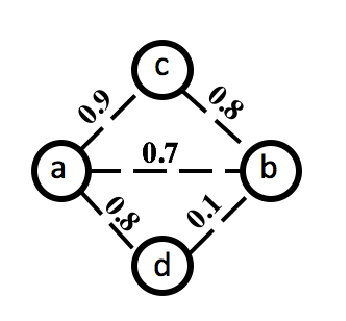
\includegraphics[scale=0.6]{figures/DegreeAUG/trueGraph.eps}
        \caption{\small{An \emph{original} graph.}}
         \label{fig:trueGraph}
    \end{subfigure}
    \begin{subfigure}[t]{0.4\textwidth}
        \centering
        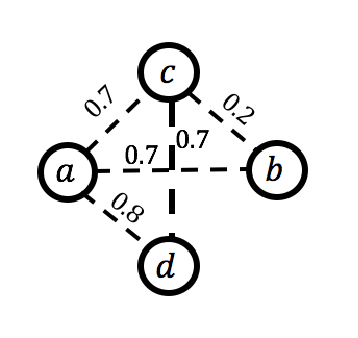
\includegraphics[scale=0.6]{figures/DegreeAUG/anGraph.eps}
        \caption{\small{An \emph{anonymization}.}}
        \label{fig:anGraph}
    \end{subfigure}
    \caption{Uncertain graph anonymization.}
    \label{fig:augExample}
\end{figure*}
As ever discussed, we want to publish the anonymized version of uncertain graphs where node identity is obfuscated enough. We adopt $\keobf$ model, proposed in \cite{Bonchi_Identity_2014}, to quantify the anonymity level achieved by an anonymized graph (uncertain graph).
Its formal definition is as follow: 
\begin{definition}
    \textbf{\boldmath{$(k,\epsilon)$}-obf \cite{Bonchi_Identity_2014}}
    Let $P$ be a vertex property, $k \geq 1$ be a desired level of anonymity, and $\epsilon >0 $ be a tolerance parameter. The uncertain graph $\tilde{\mathcal{G}}$ is said to $k$-obfuscate a given vertex $v \in V_{\mathcal{G}}$ with respect to $P$ if the entropy of the distribution $Y_{P(v)}$ over the vertices of $\mathcal{G}$ is greater than or equals to $\log_{2}{k}$:
    \vj
    \begin{equation*}
        H(Y_{P(v)}) \geq \log_{2}{k}.
    \label{obfCon}
    \svj
    \end{equation*}
The uncertain graph $\mathcal{G}$ is $(k,\epsilon)$-obf with respect to property $P$ if it $k$-obfuscates at least $(1-\epsilon)|V|$ vertices in $V_{\mathcal{G}}$. $P$ can be any node properties.  
\end{definition}

\begin{figure}[t]
        \centering    
        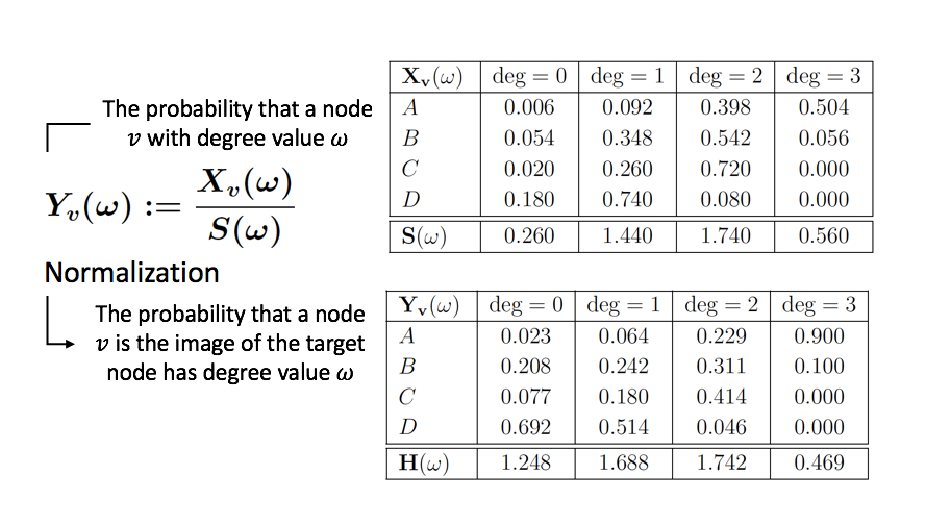
\includegraphics[scale=0.8]{figures/DegreeAUG/entropyEx.eps}
        \caption{The degree uncertainty for each node (top) and normalized values for each degree (bottom)}
    \label{fig:entropyExample}
\end{figure}

\emph{Figure \ref{fig:entropyExample}  gives an example of how to compute degree entropy for the uncertain graph in Figure \ref{fig:trueGraph}. Each row in the top side is the degree distribution for the corresponding node. For example, node $a$ has degree $0$ with probability $(1-0.9)(1-0.8)(1-0.7)=0.006$. The last row in the top side is the sum of probability over all the nodes. For example, $S(0)=0.006+0.054+0.020+0.180=0.26$.
The bottom one normalizes values in each column to get distribution $Y_{P(v)}$. For example, $Y_{0}(a)$= $\frac{X_{0}(a)}{S(0)}=0.023$. The entropy $H(Y_d(v))$ for each degree value $\omega$ is shown in the last bottom row. Given $k=3, \log_{2}{3}=1.58$, node $b,c$ with expected degree $2$ and $d$ with true degree $1$ satisfies $k$-obf while $a$ with expected degree $3$ fails, thus $\epsilon=0.25$. }

\subsection{Reliability-based Utility Criteria}
Inspired by the importance of reliability, we suggest to quantify the utility loss, anonymization cost, as the reliability difference between the anonymized result $\tilde{\mathcal{G}}$ and the original one $\mathcal{G}$, reliability discrepancy. We proceed to explain its formal definition. 

In the context of uncertain graphs, \emph{reliability} generalizes the concept of connectivity by  capturing the probability that two given (sets of) nodes are reachable over all possible worlds. We focus on two-terminal reliability. 
\begin{definition}
    \textbf{Two-Terminal Reliability \cite{Colbourn_Colbourn_1987}}  Given an uncertain graph $\mathcal{G}$, and two distinct nodes $u$ and $v$ in $V$, the reliability for two nodes $(u,v)$ is defined as follows:
        \vj
        \begin{equation*}
                R_{u,v}(\mathcal{G})= \sum_{G \subseteq W(\mathcal{G})}  \mathcal{I}_{G}(u,v) Pr[G] 
        \svj
        \end{equation*}
     
    where $\mathcal{I}_{G}(u,v)$ is 1 when $u$ and $v$ are contained in a connected component in $G$, and 0 otherwise.     
    \label{d:reliability}
\end{definition}

\begin{definition}
    \textbf{Two-Terminal Reliability Discrepancy}
    The reliability discrepancy of two distinct nodes $(u,v)$ is defined as the absolute difference of  corresponding reliability values in the original graph $\mathcal{G}$ and the anonymized result $\tilde{\mathcal{G}}$. Its formal definition is as follows:  
    \begin{equation*}
    RD_{u,v}(\tilde{\mathcal{G}})= |R_{u,v}(\mathcal{G})-R_{u,v}(\tilde{\mathcal{G}})|
    \end{equation*}
\end{definition}
Thus, we come up the definition of reliability discrepancy of the overall anonymized result against the true graph.   
\begin{definition}
    \textbf{Reliability Discrepancy}
    Compared to the input uncertain graph $\mathcal{G}=(V,E,\mathit{p})$, the reliability discrepancy of one anonymized instance $\tilde{\mathcal{G}}=(V,E, \tilde{\mathit{p}})$ is the sum of $RD$ over all vertex pair $(u,v)$. The formal definition is as follows: 
    \begin{equation*}
        \Delta(\tilde{\mathcal{G}})=\sum_{(u,v)} RD_{u,v}(\tilde{\mathcal{G}})
    \end{equation*}
\end{definition}

\begin{example}
 Given an input uncertain graph $\mathcal{G}$ in Figure \ref{fig:trueGraph} and its anonymization $\tilde{\mathcal{G}}$ in Figure \ref{fig:anGraph} and suppose one wants to compute $RD_{a,b}(\tilde{\mathcal{G}})$. Following the definition,  the reliability of node pairs $(a,b)$ for $\mathcal{G}$ in Figure \ref{fig:trueGraph} equals 0.92272. While, the \emph{reliability} of node pairs in Figure \ref{fig:anGraph} equals $0.75208$. Thus, the \emph{reliability discrepancy} of node pair $RD_{a,b}(\tilde{\mathcal{G}})$ is $|0.92272-0.75208|=0.17064$. 
\end{example}

We are ready to formulate the problem, reliability preserving anonymization in the context of uncertain graphs. 
\begin{problem}
     \textbf{Reliability Preserving Anonymization over Uncertain graphs}
     Given an uncertain graph $\mathcal{G}=(V,E,\mathit{p})$ and anonymization parameters $k, \epsilon$, the objective is to find a possible $(k,\epsilon)$-obfuscated graph $\tilde{\mathcal{G}}=(V,E,\tilde{\mathit{p}})$ with minimal reliability discrepancy  $\Delta(\tilde{\mathcal{G}})$, as
     \begin{equation*}
             \begin{aligned}
                 & \argmin_{\tilde{
                \mathcal{G}}} & & \Delta(\tilde{\mathcal{G}}) \\
                &  \text{Subject to} & &\tilde{\mathcal{G}} \text{~is~} (k,\epsilon)-obf
            \end{aligned}
     \end{equation*}
     \label{prob:unobf}
\end{problem}

\chapter{Distributed Triangle Listing Algorithm}
\label{chp:bec}
In this chapter, I will briefly review the distributed triangle listing techniques I developed for MapReduce Framework. These techniques have been submitted as a conference paper \cite{}.

In this work, we present Bermuda method which effectively reduces the size of the intermediate data via redundancy elimination and sharing of messages whenever possible. As a result, Bermuda achieves orders-of-magnitudes of speedup and enables processing larger graphs that other techniques fail to process under the same resources. Bermuda exploits the locality of processing, i.e.,  in which reduce instance each graph vertex will be processed, to avoid the redundancy of generating messages from mappers to reducers. Bermuda also proposes novel message sharing techniques within each reduce instance to increase the usability of the received messages. 

\section{Overview}
\label{sec:bectech}
With the MR-Baseline Algorithm, one node needs to send the same pivot message to multiple nodes residing in the same reducer. Therefore, the network traffic can be reduced by sending only one message to the destination reducer, and either have main-memory cache or distributing the message 
to actual graph nodes within each reducer. Although this strategy seems quite simple, and other systems such as GPS and X-Pregel~\cite{X-Pregel,GPS} have implemented it, the trick lies on how to efficiently perform the caching and sharing. In this section, we propose new effective caching strategies to maximize the sharing benefit while encountering little overhead. We also present novel theoretical analysis for the proposed techniques. 

In the frameworks of GPS and X-Pregel, adjacency lists of high degree nodes are used for identifying distinct destination reducer and distributing the message to target nodes in the reduce side. This method requires extensive memory and computations for message sharing.  
In contrast, in Bermuda, each node uses the {\em universal key partition function} to group its destination nodes. Thus, each node would only send the same pivot 
message to each reduce instance only once. 
At the same time, reduce instances will adopt different message-sharing strategies to guarantee the correctness of algorithm. 
As a result,  Bermuda achieves a trade off between reducing the network communication---which is known to be a big bottleneck for map-reduce jobs---and increasing the processing cost and memory utilization. 

\section{Bermuda Edge-Centric Node++ }
\label{sec:EC}
A straightforward (and intuitive) approach for sharing the pivot messages within each reduce instance 
is to organize either the pivot or core messages in main-memory for efficient random access. 
We propose the Bermuda Edge-Centric Node++ (Bermuda-EC) algorithm,  which is based on the observation that for a given input graph, 
it is common to have the number of core messages smaller than the number of pivot messages. 
Therefore, the main idea of Bermuda-EC algorithm is to first read the core messages, cache them in memory, and then stream the pivot messages, 
and on-the-fly intersect the pivot messages with the needed core messages (See Figure~\ref{fig:Bermuda-EC}). 
The MapReduce code of the Bermuda-EC algorithm is presented in Algorithm~\ref{alg:Bermuda-EC}.
% For the purpose of reducing 

In order to avoid pivot message redundancy, a universal key partitioning function is utilized by mappers. 
The corresponding modification in the map side is as follows. First, each node $v$ employs a universal key partitioning function $h()$ to group its destination nodes 
(Line 3, Algorithm \ref{alg:Bermuda-EC}). This grouping captures the graph nodes that will be processed by the same reduce instance. 
Then, each node $v$ sends a pivot message including the information of $N_v^H$ to each non-empty group (Lines 4-6, Algorithm \ref{alg:Bermuda-EC}). 
Following this strategy, each reduce instance receives each pivot message exactly once even if it will be referenced multiple times. 

Moreover, we use tags to distinguish core and pivot messages, which are not listed in the algorithm for simplicity.  
Combined with the MapReduce internal sorting function, Bermuda-EC guarantees that all core messages are received by the reduce function before any of the pivot messages 
as illustrated in Figure \ref{fig:Bermuda-EC}. 
Therefore, it becomes feasible to cache only the core messages in memory, and then perform the intersection as the 
pivot messages are received.

The corresponding modification in the reduce side is as follows. For a given reduce instance $R_i$, it first reads all the core message into main-memory (Line 7, Algorithm \ref{alg:Bermuda-EC}). Then, it iterates over all pivot message. Each pivot message is  intersected with the cached core messages for identifying the triangles. 
As presented in the MR-Baseline algorithm (Algorithm~\ref{alg:MR-Baseline}), each pivot message $(v,N_v^H)$ needs to be processed in reduce instance $R_i$ only for 
nodes ${u: u \in N_v^H ~ where~ h(u)=i}$. Interestingly, this information is  encoded within the pivot message. Thus, each pivot message is processed for all its requested core nodes once received 
(Lines 9-11, Algorithm \ref{alg:Bermuda-EC}). 
%Summing up all pivot messages, reduce instance $R_i$ recover the total work. 
%
%By default, the key partitioning function is a hash function over node ID {\ie}, $h(v) \in [0,k-1]$ where $k$ equals the number of reducers. 
%Hash function is a good choice of universal key partition function for its light encoding cost and computation overhead. 

\begin{algorithm}[tb]
	\begin{algorithmic}[1]
			\item[] \textbf{Map}: Input:($ \langle v; N_v^H \rangle$) 
            \item[] {Let $h(.)$ be a key partitioning function into [0,k-1] }
			\STATE $j \leftarrow h(v)$
			\STATE emit $\langle j;(v,N_v^H) \rangle$
			\STATE \emph{Group} the set of nodes in $N_v^H$ by $h(.)$
			\FORALL {$i \in [0,k-1]$}
				\IF {$gp_i \neq \emptyset$}
					\STATE emit $\langle i;(v,N_v^H) \rangle$
				\ENDIF
			\ENDFOR
            \item[]
			\item[] \textbf{Reduce}:Input:$[\langle i;(v,N_v^H) \rangle]$ 
			\STATE initiate all the core nodes' $N_u^H$ in main memory
            \FORALL {pivot message $\langle i;(v,N_v^H) \rangle $}
                \FORALL {$u \in N_v^H $ and $h(u)=i$}
                    \FORALL {$w \in N_v^H \cap N_u^H $}
                        \STATE emit $\triangle_{vuw}$
                    \ENDFOR
            \ENDFOR
			\ENDFOR
			\end{algorithmic}
		\caption{Bermuda-EC}
		\label{alg:Bermuda-EC}
\end{algorithm}
\begin{figure}[t]
		\centering	
        \includegraphics[scale=0.4]{figures/bermuda/BENode++2.eps}
		\caption {\small{Bermuda-EC Execution.}}
		\label{fig:Bermuda-EC}
\end{figure}



\subsubsection{Analysis of Bermuda Techniques}
\label{sec:ECAnalysis}
Extending  the analysis in Section \ref{sec:MR_baseline}, we demonstrate that Bermuda-EC achieves improvement over MR-Baseline w.r.t both space usage and execution efficiency. 
Furthermore, we discuss the effect of the number of reducers  $k$ on the algorithm performance.

\begin{theorem}
\label{th:ECsize}
	For a given number of reducers $k$, we have:
    \begin{itemize}
    	\item {The expected total size of the map output is $O(km)$}.
        \item {The expected size of core messages to any reduce instance is O(m/k)}. 
    \end{itemize}
\end{theorem}

\begin{proof}
	As shown in Algorithm \ref{alg:Bermuda-EC},  the size of the map output generated by node $v$ is at most $k*\hat{d_v}$.  Thus, the total size of the map output $T$ is as follows:
    \vj
    \[ T < \sum_{v \in V} k \hat{d_v} = k \sum_{v \in V} \hat{d_v}= km \]
    For the second bound, observe that a random edge is present in a reduce instance $R_i$ and represented as a core message with probability $1/k$.    
     By following the {\em Linearity of Expectation}, the expected number of the core messages to any reduce instance is $O(m*\frac{1}{k})$. 
\end{proof}

\textbf{Space Usage.} Theorem~\ref{th:ECsize} shows that when $k \ll \sqrt[]{m}$ (the usual case for massive graphs), 
then the total size of the map output generated by Bermuda-EC algorithm is significantly 
less than that  generated by the MR-Baseline algorithm. In other words, Bermuda -EC is able to handle even larger graphs with limited compute clusters. 
%A detailed experimental comparison with MR-Baseline is given in the experiment section.
\textbf{Execution Time.} A positive consequence of having a smaller intermediate result is that it requires less time for generating and shuffling/sorting the data. 
Moreover, the  imbalance of the map outputs is also reduced significantly by limiting the replication factor of the pivot messages up to $k$.
The next theorem shows the approximate variance of the number of the intermediate result from mappers. 
When $k < E(x)$, it implies smaller variance among the mappers than that of the MR-Baseline algorithm. 
Together, Bermuda -EC achieves better performance and scales to larger graphs compared to the MR-Baseline algorithm. 

\begin{theorem}
\label{th:BEC}
	For a given graph $G(V,E)$, let a random variable x denotes the effective degree of any node in $G$ and the variance of x is denotes as Var(x). Then the expectation of x ($E(x)$) equals the average degree and computed as $E(x)=\frac{m}{n}$. For typical graphs, $Var(x) \neq 0$ and $E(x) \neq 0$ always hold. Since each mapper starts with approximately the same input size (say receives $c$ graph nodes), the variance of the map output's size under the Bermuda-EC Algorithm is  $O(2ck^2Var(x))$, 
	where $k$ represents the number of reducers. 
\end{theorem}

\begin{proof}    
    Assume the number of reducers is $k$. Given a graph node $v$, where its effective degree $\hat{d_v}=x$. 
    Let random variable $y(x)$ be the number of distinct reducers processing the effective neighbors of $v$, and thus  $y(x) \leq k$. 
    Then, the size of the map output generated by a single node $u$ would be $xy$, denoted as $g(x)$(Lines 3-4, Algorithm \ref{alg:Bermuda-EC}). 
    Thus, the total size of the map output generated by $c$ nodes in a single mapper $T(X)=\sum_{i=1}^{c}g(x_i)$. 
    Since $x_1,x_2,..x_c$ are independent and identically distributed random variables, then $Var(T(x))=c*Var(g(x))$. 
    The approximate variance of $g(x)$ is as  follows 
    \vj
    \begin{align*}
    	Var(xy) &= E(x^2y^2)- E(xy)^2 \\
        		&< E(x^2y^2) \\
        	    &< k^2E(x^2) \\
           		&< k^2(E(x)^2+Var(x)) \\
               &< 2k^2Var(x) 
        \vspace{-4em}
    \end{align*}
As presented in \cite{Schank_2007}, $E(x^2) \approx \frac{m^{\frac{3}{2}}}{n}$ and $E(x)=\frac{m}{n}$. Thus $\frac{E(x^2)}{E(x)^2} \approx \frac{n}{\sqrt[]{m}} $. In many real graphs where $n^2 > m$ it implies $\frac{n} {\sqrt[]{m}} > \sqrt[]{m} >2$. It implies $E(x^2)> 2E(x)^2$, thus $Var(x)=E(x^2)-E(x)^2 > E(x)^2$.
\end{proof}

We now study in more details the effect of parameter $k$ (the number of reducers) on the space and time complexity for the Bermuda-EC algorithm.

\textbf{Effect on Space Usage.} The reducers number $k$ trades off the memory used by a single reduce instance and the size of the intermediate data generated during the MapReduce job. 
The memory used by a single reducer should not exceed the available memory of a single machine, {\ie}, $O(m/k)$ should be sub-linear to the size of main memory in a single machine. In addition, the total space used by the intermediate data must also remain bounded, {\ie}, $O(km)$ should be no larger than the total storage. 
Given a cluster of machines, these two constraints define the bounds of $k$ for a given 
input graph $G(V,E)$.  

\textbf{Effect on Execution Time.} The reducers number $k$ trades off the reduce computation time and the time for shuffling and sorting. 
As the parallelization degree $k$ increases, it reduces the computational time in the reduce phase. At the same time, the size of the intermediate data, {\ie}, $O(km)$ increases significantly as $k$ increases (notice that $m$ is very large), and
thus the communication cost becomes a bottleneck in the job's execution. 
Moreover, the increasing variance among mappers $O(2ck^2Var(x))$ implies a more significant straggler problem which slows down the execution progress. 

In general, Bermuda-EC algorithm favors the smaller setting of $k$ for higher efficiency while subjects to memory bound that the 
expected size of core message $O(m/k)$ should not exceed the available memory of a single reduce instance. 

Unfortunately, for processing web-scale graphs such as \emph{ClueWeb} with more than 80 billion edges (and total size of approximately 700GBs)---which as we will show the state-of-art techniques cannot actually process---the number of reducers needed  for Bermuda-EC for acceptable performance is in the order of 100s. 
Although, this number is very reasonable for most mid-size clusters, the intermediate results $O(km)$ will be huge, which leads to significant network congestion.  

\textbf{Disk-Based Bermuda-EC:} A generalization to the proposed Bermuda-EC algorithm that guarantees 
no failure even under the case where  the core messages cannot fit in a reducer's memory is the {\em Disk-Based Bermuda-EC} variation. 
The idea is straightforward and relies on the usage of the local disk of each reducer. 
The main idea is as follows: (1) Partition the core messages such that each partition fits into main memory,
 and (2) Buffer a group of pivot messages, and then iterate over the core messages one partition at a time, and for each partition, identify the triangles as in the standard Bermuda-EC algorithm. 
 Obviously, such method trades off between disk I/O (pivot message scanning) and main-memory requirement. For a setting of reduce number $k$, the expected size of core messages in a single reduce instance is $O(m/k)$, thus the expected number of rounds is $O(\frac{m}{kM})$ where $M$ represents the size of available main-memory for single reducer. The expected size of pivot message reaches $O(m)$. Therefore, the total disk I/O reaches $O(\frac{m^2}{kM})$. In the case of massive graph, it implies longer time. 

\section{Bermuda Vertex-Centric Node++} 
As discussed in Section \ref{sec:EC}, the Bermuda-EC algorithm assumes that the core messages can fit in the memory of a single reducer. However, it is not always guaranteed to be the case, especially in web-scale graphs.

One crucial observation is that the access pattern of the pivot messages
can be learned and leveraged for better re-usability. 
In MapReduce, a single reduce instance processes many keys (graph nodes) in a specific sequential order. This order is defined based on the key comparator function. 
For example, let $h()$ be the key partitioning function and $l()$ be key comparator function within the MapReduce framework, 
then $h(u)=h(w)=i$ and $l(u,w)<0$ implies that the reduce instance $R_i$ is responsible for the computations over nodes $u,~w$, and also the computations 
of node $u$ precede   that of node $w$. 
Given these known functions, the relative order among the keys in the same reduce instance becomes known,
 and the access pattern of  the pivot message can be predicted. 
The knowledge of the access pattern of the pivot messages holds a great promise for proving better caching and better memory utilization.

Inspired by these facts, we propose the~Bermuda-VC algorithm which supports random access 
over the pivot messages by caching them in main-memory while streaming in the core messages. 
More specifically, Bermuda-VC will reverse the assumption of Bermuda-EC, where we now try to make the pivot messages arrive first to reducers, 
get them cached and organized in memory, and then the core messages are received and processed against the pivot messages. 
Although the size of the pivot messages is usually larger than that of the core messages,  
their access pattern is more predictable which will enable better caching strategies as we will present in this section. 
%Moreover, \Bermuda-VC maintains the independence of distinct key/node's reduce computation as MR-Baseline algorithm. 
The Bermuda-VC algorithm is presented in Algorithm \ref{alg:Bermuda-VC}. 
\begin{algorithm}[t!]
	\begin{algorithmic}[1]
			\item[] \textbf{Map}: Input:($ \langle v;(N_v^L ,N_v^H) \rangle$) 
            \item[] {Let $h(.)$ be a key partitioning function into [0,k-1] }
            \item[] {Let $l(.)$ be a key comparator function}
			\STATE emit $\langle v;(v,N_v^L,N_v^H) \rangle$
			\STATE \emph{Group} the set of nodes in $N_v^H$ by $h(.)$
			\FORALL {$i \in [0,k-1]$}
				\IF {$gp_i \neq \emptyset$}
                	\STATE $gp_i \Leftarrow sort(gp_i) based on l(.)$
                    \STATE $u \Leftarrow gp_i.first$
					\STATE $AP_{v,i} \Leftarrow accessPattern(gp_i)$
					\STATE emit $\langle u;(v,AP_{v,i},N_v^H) \rangle$
				\ENDIF
			\ENDFOR
            \item[]
			\item[] \textbf{Reduce}:Input:$[\langle u;(v,AP_{v,i},N_v^H) \rangle]$ 
			\STATE initiate the core node $u$' $N_u^L,N_u^H$ in main memory
            \FORALL {pivot message $\langle u;(v,AP_{v,i},N_v^H) \rangle $}
            	\FORALL{$w \in N_v^H \bigcap N_u^H$}
                	\STATE emit $\triangle_{vuw}$
                \ENDFOR
                \STATE {Put $(v,AP_{v,j},N_v^H)$ into shared buffer}
                \STATE {$N_u^L\leftarrow N_u^L-\lbrace v \rbrace$}
            \ENDFOR
            \FORALL {$r \in N_u^L$}
            	\STATE {Fetch $(r,AP_{r,i},N_{r}^H)$ from shared buffer}
         		\FORALL{$w \in N_{r}^H \bigcap N_u^H$}
                	\STATE emit $\triangle_{ruw}$
               	\ENDFOR
            \ENDFOR
	\end{algorithmic}
	\caption{Bermuda-VC}
	\label{alg:Bermuda-VC}
\end{algorithm}
\begin{figure}[t]
		\centering	
		\includegraphics[scale=0.4]{figures/bermuda/BNode++.eps}
		\caption {Bermuda-VC Execution.}
		\label{fig:Bermuda-VC}
\end{figure}

% The high level idea of \Bermuda-VC algorithm is
The Bermuda-VC algorithm uses a shared buffer for  caching the pivot messages.
% Based on message sharing management, the general approach of its reduce computation is similar to MR-Baseline algorithm. 
And then, for the reduce-side computations over a core node $u$, the reducer compares $u$'s core message with all related pivot messages---some are associated with $u$'s core message, while the rest should be residing in the shared buffer. 
%
Bermuda-VC algorithm applies the same scheme to avoid generating redundant pivot messages. It utilizes a universal key partitioning function to group effective neighbors $N_v^H$ of each node $v$. 
In order to guarantee the availability of the pivot messages, a universal key comparator function is utilized to sort the destination nodes in each group (Line 5, Algorithm \ref{alg:Bermuda-VC}). As a result, destination nodes are sorted based on their processing order. The first node in group $gp_i$ indicates the earliest request of a pivot message. 
Hence, each node $v$ sends a pivot message to the first node of each non-empty group by emitting key value pairs where key equals the first node ID (Lines 6-8, Algorithm \ref{alg:Bermuda-VC}). 

Combined with the sorting phase of the MapReduce framework, Bermuda-VC guarantees the availability of all needed pivot messages of any node $u$ when $u$'s core message is received by a reducer, i.e.,  the needed pivot messages are either associated with $u$ itself or associated with another nodes processed before $u$. 

The reducers' processing mechanism is similar to that of  the MR-Baseline algorithm. 
Each node $u$ reads its core message for initiating $N_u^H$ and $N_v^L$ (Line 9), and then it iterates over every pivot message associated with key $u$ against its effective adjacency list $N_v^H$ to enumerate the triangles (Lines 10-12). As discussed before, not all expected pivot messages are carried with key $u$. 
The rest of the related pivot messages reside in the shared buffer. Here, $N_v^L$ is used for fetching the rest of these pivot 
messages (Line 14, Algorithm \ref{alg:Bermuda-VC}), and enumerating the triangles (Lines 15-18, Algorithm \ref{alg:Bermuda-VC}). 
Moreover, the new coming pivot messages associated with node $u$ are pushed into the shared buffer for further access by other nodes (Line 13). 
Figure \ref{fig:Bermuda-VC} illustrates the reduce-side processing flow of Bermuda-VC. 
In the following sections, we will discuss in more details the management of the pivot messages in the shared buffer.
%Its appeal stems from the fact that the reduce computation of different keys/nodes is isolated. While, it requires random access to pivot messages which may not fit in main-memory for massive graphs. To solve this problem, we introduce different message sharing management schemes as described next. 

\subsection{Message Sharing Management}
Note that, each reduce instance uses its shared buffer to organize sharing pivot messages in memory. Message sharing via shared buffer is effective because the reduce computation program access the same pivot message over and over. By keeping as much of  pivot message as possible in the shared buffer, it avoids access the slower medium--disk. 
In general, there are two types of operations over the shared buffer inside a reduce instance, which are: {\em ``Put''} for adding new incoming pivot messages into the shared buffer (Line 13), and {\em ``Get''} for retrieving  the needed pivot messages (Lines 15-18).  For massive graphs, the main memory may not hold all the pivot messages.  
This problem is similar to the classical caching problem studied in~\cite{keramidascache2007, petoumenos2009}, where a {\em  reuse-distance} factor is used to estimate the distances between consecutive references of a given cached element, and based on that effective  replacement policies can be deployed. We adopt the same idea in  Bermuda-VC.

Interestingly, in addition to the reuse distance, all access patterns of each pivot message can be easily estimated in our context.
The access pattern $AP$ of a pivot message is defined as the sequence of graph nodes (keys) that will reference this message. 
In particular, the access pattern of a pivot message from node $v$ to reduce instance $R_i$ can be computed based on the sorted effective nodes $gp_i$ received by $R_i$. Several interesting metrics can be derived from this access pattern. 
For example, the first node in $gp_i$ indicates the occurrence of the first reference, the size of $gp_i$ equals the cumulative reference frequency. 
Such access pattern information is encoded within each pivot message (Lines 7-8, Algorithm \ref{alg:Bermuda-VC}). 
With the availability of this access pattern, effective message sharing strategies can be deployed under limited memory.  

\begin{figure}[t]
		\centering	
		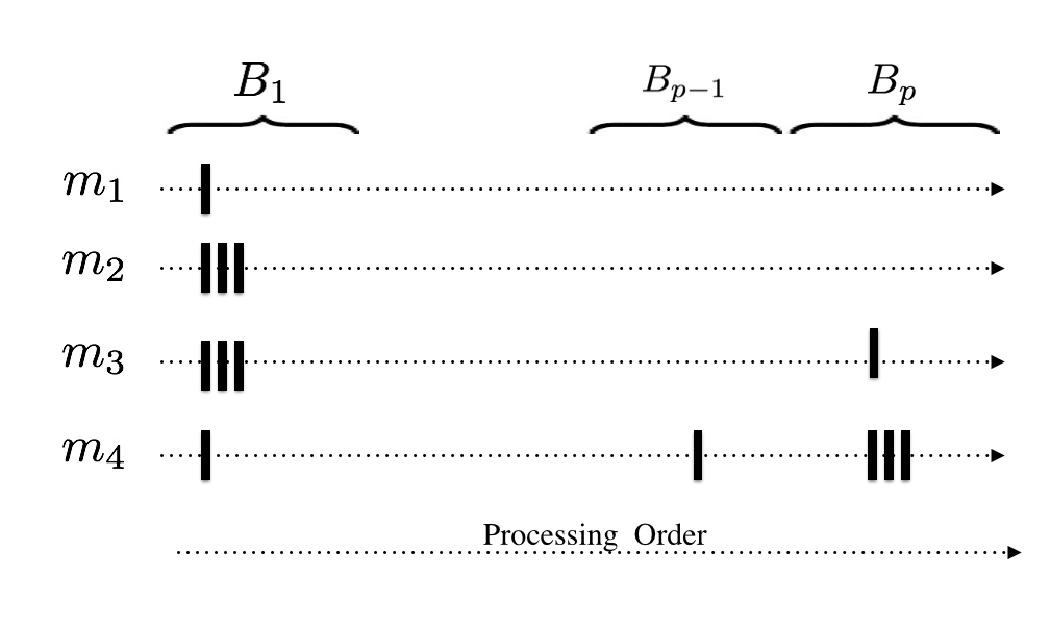
\includegraphics[scale=0.4]{figures/bermuda/usagePattern.eps}
		\caption {Various access Patterns for Pivot Messages.}
		\label{fig:upattern}
\end{figure}

As an illustrative example, Figure \ref{fig:upattern} depicts different access patterns for four pivot messages \{$m_1,~m_2,~m_3,~m_4$\}. 
The black bars indicate requests to the corresponding pivot message, while the gaps represent the re-use distances (which are idle periods for this message). 
Pivot messages may exhibit entirely different access patterns, e.g., pivot message $m_1$ is referenced only once, while others are utilized more than once, and some pivot messages are used in dense consecutive pattern in a short interval, {\eg}, $m_2$ and $m_3$. 
%
Inspired by these observations, we propose two heuristic-based replacement policies, namely \emph{usage-based tracking}, and \emph{bucket-based tracking}. 
They trade off the tracking overhead with memory hits as will be described next. 


\hspace{-2em}
\textbf{$\bullet$Usage-Based Tracking}
Given a pivot message originated from node $v$, the total use frequency is limited to $\sqrt[]{m}$, referring to the number of its effective neighbors, which is much smaller than the expected number of nodes processed in a single reducer, which is estimated to $n/k$. This  implies that each pivot message may become useless (and can be discard) as a reducer progresses, and it is always desirable to detect the earliest time at which a pivot message can be discarded to maximize the  memory's utilization.

The main idea of the usage-based tracking is to use a usage counter per pivot message in the shared buffer. And then, the tracking is performed as follows. Each \emph{Put} operation sets the counter as the total use frequency. And, only the pivot messages whose usage counter is larger than zero are added to the shared buffer. Each \emph{Get} operation decrements the counter of the target pivot message by one. Once the counter reached zero, the corresponding pivot message is evicted from the shared buffer. 

The usage-based scheme may fall short in optimizing sparse and scattered access patterns. For example, as shown in Figure~\ref{fig:upattern}, the reuse distance of message $m_4$ is large. Therefore, the usage-based tracking strategy has to keep $m_4$ in the shared buffer although it will not be referenced for a long time. What's worse, such  scattered access is common in massive graphs. Therefore,  pivot messages may unnecessarily overwhelm the available memory of each single reduce instance.  

\hspace{-2em}
\textbf{Bucket-Based Tracking}
We introduce the \emph{Bucket-based} tracking strategy to optimize message sharing over scattered access patterns. The main idea is to manage the access patterns of each pivot message at a smaller granularity, called a {bucket}. The processing sequence of keys/nodesis sliced into buckets as illustrated in Figure \ref{fig:upattern}. 
In this work, we use the range partitioning method for balancing workload among buckets. 
Correspondingly, the usage counter of one pivot message is defined per bucket, i.e., each message will have an array of usage counters of a length equals to the number of its buckets. 
For example, the usage count of $m_4$ in the first bucket is $1$ while in the second bucket is $0$. 
Therefore, for a pivot message that will remain idle (with no reference) for a long time, its counter array will have a long sequence of adjacent zeros. Such access pattern information can be computed in the map function, encoded in access pattern (Line 7 in Algorithm~\ref{alg:Bermuda-VC}), and passed to the reduce side. 

\begin{figure}[t]
		\centering	
		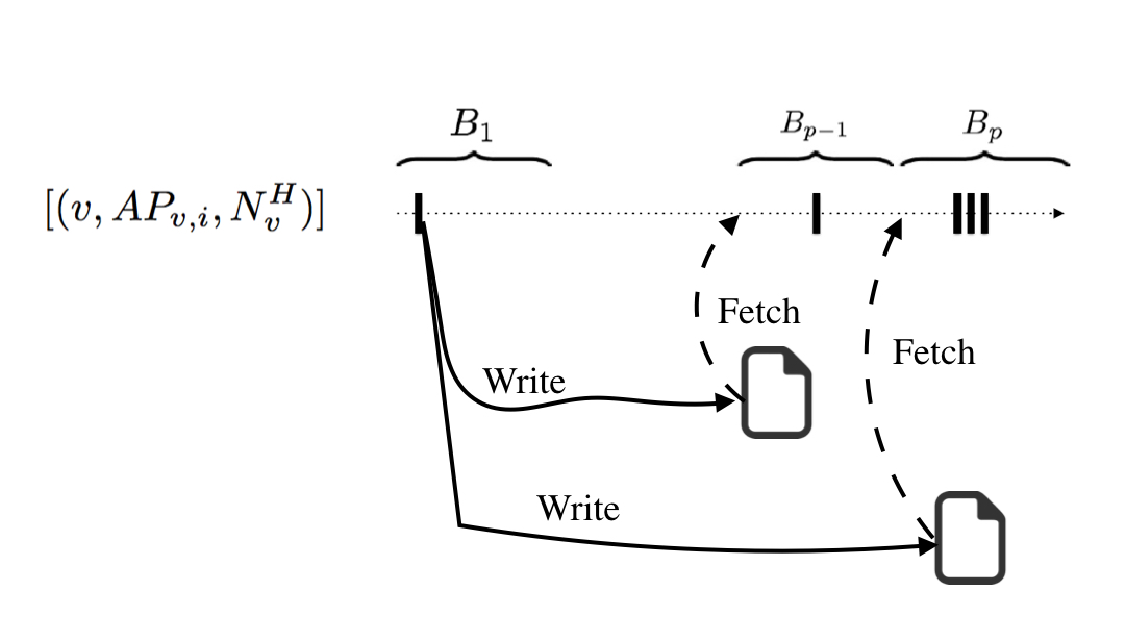
\includegraphics[scale=0.4]{figures/bermuda/bucketFetching.eps}
		\caption {Read and Write Back-up files}
		\label{fig:bucketFetch}
\end{figure}

The corresponding modification of the \emph{Put} operation is as follows.  Each new pivot message will be pushed into the shared buffer (in memory) and backed up by local files (in disk) based on its access pattern. 
Figure \ref{fig:bucketFetch} illustrates this procedure. For the arrival of a pivot message with the access pattern $[1,0,.., 1,3]$, the reduce instance actively adds this message into back-up files for buckets $B_{p-1}$ (next-to-last bucket) and $B_{p}$ (last bucket). And then, at the end of each bucket processing and before the start of processing the next bucket, 
all pivot messages in the shared buffer are discarded, and a new set of pivot messages is fetched from the corresponding back-up file into memory(See Figure \ref{fig:bucketFetch}). 

The Bucket-based tracking strategy provides better memory utilization since it prevents the long retention of unnecessary pivot messages. In addition, usage-based tracking  can be applied to each bucket to combine both benefits,  which is referred to as the {\em bucket-usage} tracking strategy. 

\subsection{Disscussion}
In this section, we show the benefits of the Bermuda-VC algorithm over the Bermuda-EC algorithm. 
Furthermore, we discuss the effect of  parameter $p$, which is the the number of buckets, on the performance.

Under the same settings of the number of reducers $k$, the Bermuda-VC algorithm generates more intermediate message and takes longer execution time.  Firstly, the Bermuda-VC algorithm generates the same number of pivot messages while generating more core messages ({\ie}, additional $N_v^L$ for reference in the reduce side).
Thus, the total size of the extra $N_v^L$ core message is $\sum_{v \in V} N_v^L=m$. 
Such noticeable size of extra core messages requires additional time for generating and shuffling. 
Moreover, an additional computational overhead (Lines 13-14) is required for the message sharing management. 

However, because of the proposed sharing strategies, the Bermuda-VC algorithm can work under smaller settings for $k$---which are settings under which the Bermuda-EC algorithm will probably fail.  In this case, the benefits brought by having a smaller $k$  will exceed the corresponding cost. In such cases, Bermuda-VC algorithm will outperform Bermuda-EC algorithm. 

Moreover, compared to the disk-based Bermuda-EC algorithm, the Bermuda-VC algorithm has a relatively smaller disk I/O cost because the predictability of the access pattern of the pivot messages, which enable purging them early, while that is not applicable to the core messages. Notice that, for any given reduce instance, the expected usage count of pivot message from $u$ is $d_u^H/k$. Thus, the expected usage count for any pivot message is $E(d_u^H)/k$, equals $m/nk$.  Therefore, the total disk I/O with pivot messages is at most $m^2/nk$, smaller than disk I/O cost of Bermuda-EC algorithm $m^2/Mk$, where $M$ stands for the size of the available memory in a single machine.

{\textbf{ Effect of the number of buckets $p$: }} At a high level, $p$ trades off the space used by the shared buffer with the I/O cost for writing and reading the back-up files. Bermuda-VC algorithm favors smaller settings of $p$ in the capacity of main-memory. As $p$ decreases, the expected number of reading and writing decreases, however the total size of the pivot messages in the shared buffer may exceed the capacity of the main-memory. 
For a setting of $p$, the expected size of the pivot messages for any bucket is $O(m/kp)$. Therefore, a visible solution for $O(m/kp) \le M$ is $ \ge O(m/kM)$. 
Here, $p$ is set as $O(m/kM)$ where $m$ is the size of the input graph, and $M$ is the size of the available memory in a single machine. 



\chapter{Degree Anonymization over Uncertain Graphs}
\label{chp:d}
In this chapter, I will briefly review the degree anonymization tehcniques I developed for uncertain graphs. These techniques have been submitted as a conference paper \cite{}.

In this work, we study the novel problem of anonymization in the context of uncertain graphs. We extend the existing framework to work over uncertain graph by integrating uncertainty into anonymization process. In particular, we introduce a new {\em reliability-based} utility metric suitable for uncertain graphs, in contrast to the existing metrics which are all geared towards deterministic graphs. We present an efficient approach which achieves the desired level of anonymity at a slight cost of reliability by perturbing edge uncertainties judiciously.  To this purpose, we develop two uncertainty-aware heuristics based on the uncertain graph theory, which is {\em reliability-oriented}~edge selection and {\em anonymity-oriented} edge perturbing.  We show that the incorporation of uncertainty is necessary and beneficial. We experimentally evaluate the proposed approach using different real-world datasets and study the behavior of the algorithms under the different heuristics.  The results demonstrate the effectiveness of our approach. 

\section{Naive Approach: Anonymization via Representative Instance}
\label{sec:repOB}
\begin{figure}[t]
    \centering  
        \includegraphics[scale=0.38]{figures/DegreeAUG/repOB.eps}
    	\caption{Illustration of anonymizing an uncertain graph though its representative deterministic instance and its drawback.}
    \label{fig:repOB}
\end{figure}
A naive approach of anonymizing an uncertain graph is to first somehow transform it to a deterministic graph, then perform anonymization processing over the deterministic one. Fortunately, an increasing research effort was dedicated to the topic of exacting representative deterministic graphs from an uncertain graph \cite{Parchas_Gullo_Papadias_Bonchi_2014}. Parchas  {\etal} \cite{Parchas_Gullo_Papadias_Bonchi_2014} ever introduced algorithms for extracting deterministic representative graph which captures key properties of the input uncertain graph. Now, it becomes realizable to anonymize an uncertain graph in two steps as shown in Figure \ref{fig:repOB}. We first extract one deterministic representative instance $G$ from the input uncertain graph $\mathcal{G}$. Then, we anonymize the extracted deterministic graph $G$, and output this result as the anonymized result of the original uncertain graph $\mathcal{G}$ (referred as {\repAn}). 

The {\repAn} approach is attracting since it does not require any new anonymization techniques specific designed for uncertain graphs. When the extracted representative deterministic graph $G$ is close enough to the input uncertain graph $\mathcal{G}$ in terms of graph properties, its anonymized result is expected to be a good anonymization of the input uncertain one. However, there is a non-negotiable difference between the input uncertain graph $\mathcal{G}$ and its deterministic representative instance $G$, as exemplified in Figure \ref{fig:repOB}. The anonymized result of $G$ which is structurally similar to itself instead of the input uncertain graph, consequently, may be far different from the optimal solution, as exemplified in Figure \ref{fig:repOB}. Therefore, we believe that for many applications, the {\repAn} approach,  introducing a high level of noise in such fashion, do reduce the overall graph utility.  In experiment section, we will further illustrate this phenomenon over real-world datasets. 
\begin{sloppypar}
\section{Reliability-Preserving anonymization on uncertain graphs}
\end{sloppypar}
\label{sec:tech} 
In this section, we first give a brief review of the state-of-art framework which anonymizes deterministic graphs by injecting uncertainty to certain edges. Then, we discuss how to extend this framework to work over uncertain graphs by explicitly incorporating edge uncertainty.  
\begin{algorithm}[!t]
	\begin{algorithmic}[1]
    	\item[] {\textbf{Input:}~Uncertain graph $\mathcal{G}$, adversary knowledge $ak$, obfuscation level $k$, tolerance level $\epsilon$, size multiplier $c$ and white noise level $q$ }
        \item[] {\textbf{Output:}~The anonymized result $\tilde{\mathcal{G}}_{f}$}
        \STATE {Initiation of an lower bound $\sigma_{l}$ and an upper bound $\sigma_{u}$}
        \WHILE{(not terminated)}
        	\STATE {Search of $(k,\epsilon)$-obf using standard deviation $\sigma$ \\ 
            $\langle \tilde{\epsilon}, \tilde{\mathcal{G}}  \rangle$ $\leftarrow$ \texttt{GenerateObfuscation($\mathcal{G}$,$\sigma_{u}$,$ak$,$k$,$\epsilon$,$c$,$q$)}}
            \STATE {Update the anonymized result if necessary}
            \STATE {Update the lower bound or the upper bound}
            \STATE {Update the size multiplier $c$ if necessary}
        \ENDWHILE
        \STATE{return the anonymized result $\tilde{\mathcal{G}}_{f}$}
        \caption{Anonymization over uncertain graphs}
    	\label{alg:binarySearch}
    \end{algorithmic}
\end{algorithm}
\subsection{Anonymization Procedure}
% \input{mainRoutine.tex}
% \begin{figure}[!tb]
%         \centering
%          \includegraphics[scale=0.38]{figures/binarysearch.eps}
%          \caption{\small{Uncertain Graph Anonymization Flowchart }}
%         \label{fig:binarySearch}
% \end{figure}
\begin{figure*}[!tb]
    \centering
    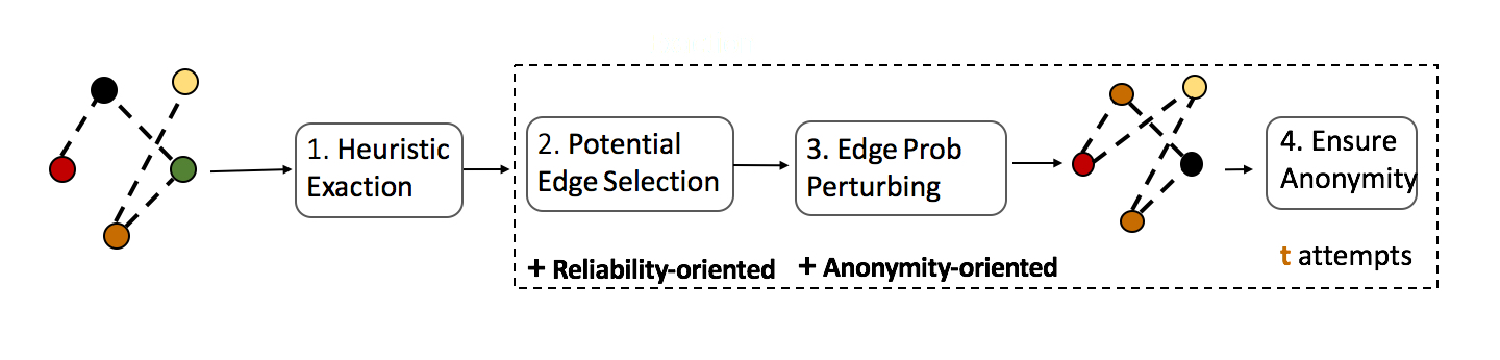
\includegraphics[scale=0.55]{figures/DegreeAUG/pipeline.eps}
    \caption{The pipeline of function \texttt{GenerateObfuscation}}
    \label{fig:genObfuscation}
\end{figure*}

Boldi {\etal}  proposed a seminal approach of anonymizing \emph{deterministic graphs} which injects uncertainty in the existence of the edges of the graph and publishes the resulting \emph{uncertain graph}. Their method injects uncertainty to edges in a deterministic graph as follows: for each existing sampled edge $e$, it is assigned a probability $1-r_{e}$, and for each non-existing sampled edge $e$, it is assigned a probability $r_{e} \leftarrow R_{\sigma_{e}}$.  By this way, it converts the input graph into an uncertain one. In particular, the perturbation variable $r_{e}$ is generated by a truncated $[0,1]$ normal distribution, $r_{e} \leftarrow R_{\sigma_{e}}$; 
\begin{equation*}
    R_{\sigma}(r):= \begin{cases}
                    \frac{\Phi_{0,\sigma}(r)}{\int_{0}^{1} \Phi_{0,\sigma}(x) dx} &  r \in [0,1] \\
                    0 &  \text{otherwise}
                    \end{cases}
     \label{eq:gen}
\end{equation*} 
where $\Phi_{0,\sigma}$ is the density function of a Gaussian distribution. 
As the standard deviation $\sigma$ of the normal distribution decreases, a greater mass of $R_{\sigma}$ will concentrate near $r=0$ and the amount of injected uncertainty will be smaller.  Namely, smaller values of $\sigma$ contribute towards better maintaining the characteristics of the original graph. Targeting at high utility, they formulated the graph anonymization problem as the minimization of $\sigma$ and computed the minimal amount of uncertainty via a binary search on the value of the uncertainty parameter $\sigma$. The overall anonymization procedure is illustrated in Algorithm \ref{alg:binarySearch}. 

The search flow of Algorithm \ref{alg:binarySearch} is determined by the function \texttt{GenerateObfuscation}, whose pipeline is shown as Figure \ref{fig:genObfuscation}. The function \texttt{GenerateObfuscation} aims to find a $(k,\epsilon)$-obfuscation of the original \emph{graph} using a given standard deviation parameter $\sigma$. A key feature of this function is the utilization of heuristics for judicious edge selection and edge prob perturbing. The function first computes heuristics values based on node properties in the input graph. After that, the search of $\keobf$ instance starts in a randomized way: $t$ attempts are performed. Each attempt performs the following steps:
\begin{itemize}
    \setlength\itemsep{0em}
	\item{Selecting a subset of edges $E_{c}$}
    \item{Perturbing existence probabilities of selected edges}
    \item{Checking the resulting uncertain graph whether satisfies the anonymity requirement}
\end{itemize}
If the algorithm finds a $(k,\epsilon)$-obfuscated graph in one of its $t$ trials, it returns the obfuscated graph with minimal $\epsilon$. Otherwise, the algorithm indicates the failure by returning $\tilde{\epsilon}=1$. 

\begin{sloppypar}
In this work, we extend this broad framework by incorporating its key function \texttt{GenerateObfuscation} with uncertainty. The specific method proposed in \cite{Boldi_Injecting_2012}, has two drawbacks for anonymizing uncertain graphs. First, their method does not consider the structural relevance of edges in the critical edge selection step, which leads to unnecessary structural distortion. Second, its interior edge perturbing mechanism assumes the existence of edges is known with certainty, thus fails to handle uncertain graphs where the existence of edges is probabilistic. We will present corresponding solutions (reliability-oriented edge selection and anonymity-oriented edge perturbing). 
\end{sloppypar}
\subsection{Reliability-oriented Edge Selection} 
\begin{sloppypar}
The most important step is the selection of potential edges, which impacts further anonymization effort significantly. Finding the optimal set of edges $E_{c}$ that balances privacy and utility is a typical combinational optimization problem. The problem is computationally expensive since there are exponential many combinations to be considered.     

To alleviate the combinational intractability, kind of heuristics have been utilized in the context of deterministic graphs. These heuristics can be classified into two main categories  (1) Anonymity-oriented ones that suggest implementing larger perturbation to less anonymized nodes~\cite{Ying2009} (2) Utility-oriented ones that suggest implementing smaller perturbation to more influential edges/nodes~\cite{casasprivacy,Ying_Randomizing_2008}. 
\end{sloppypar}

In this work, we present a sampling-based approach which combines both heuristics together. First, we adopt the idea of \emph{uniqueness score} for quantifying the anonymity level of nodes. Second, we introduce a novel edge relevance metric, \emph{reliability relevance} (RR), for quantifying the impact of edge modification to the overall uncertain graph. In contrast to the existing metrics such as edge betweenness~\cite{casasprivacy}, which are all defined in deterministic graphs, reliability relevance geared towards uncertain graphs. It allows us to select a subset of edges subjected to perturbation with less impact on reliability (reliability-oriented edge selection). 

\subsubsection{Uniqueness Score}
\label{sec:uniqueness}

\emph{Uniqueness score} is proposed to measure how typical the node is among all the nodes in terms of its property value \cite{Boldi_Injecting_2012}. More formally, the uniqueness score is defined as follows. 
\begin{definition}
    \textbf{Uniqueness Score~\cite{Boldi_Injecting_2012}}
     Let $P:V \rightarrow  \Omega_{P}$ be a property on the set of nodes $V$ of the graph $\mathcal{G}$, let $d$ be a distance function on $\Omega_{P}$, and let $\theta >0$  be a parameter. 
  Then the $\theta-commonness$ of the property values $\omega \in \Omega_{P}$ is $C_{\theta}(\omega):= \sum_{u \in V} \Phi_{0,\theta}(d(\omega, P(v)))$,   
while the $\theta$-uniqueness of $\omega \in \Omega_{P}$ is $U_{\theta}:= \frac{1}{C_{\theta}(\omega)}$. 
\end{definition} 
Note that, the commonness of the property value $\omega$ captures how typical the value $\omega$  is among all the  nodes in the graph via a weighted average function, where the weight decays exponentially as the distance $d$. As above defined, uniqueness scores depend on the parameter $\theta$, which determines the decay rate of average weights. In this work, we set $\theta=\sigma_{\mathcal{G}}$, where $\sigma_{\mathcal{G}}$ represents how frequently the property value spread in the uncertain graph $\mathcal{G}$. A comprehensive discussion can be found in the literature \cite{Boldi_Injecting_2012}.

\subsubsection{Reliability Relevance}

\begin{figure}[!tb]
    \begin{subfigure}[b]{0.45\textwidth}
        \centering
         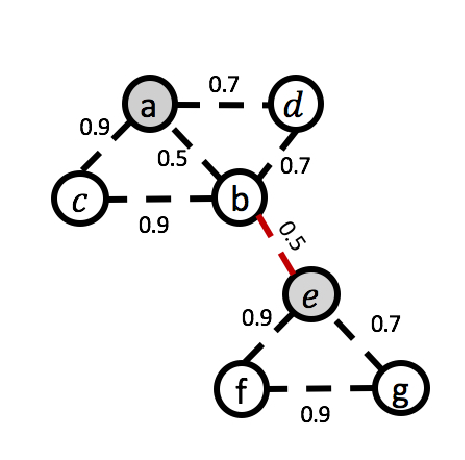
\includegraphics[scale=0.4]{figures/DegreeAUG/uncertainO.eps}
         \caption{\small{An uncertain graph}}
        \label{fig:edgeBridgeGraph}
    \end{subfigure}
    \begin{subfigure}[b]{0.45\textwidth}
        \centering
         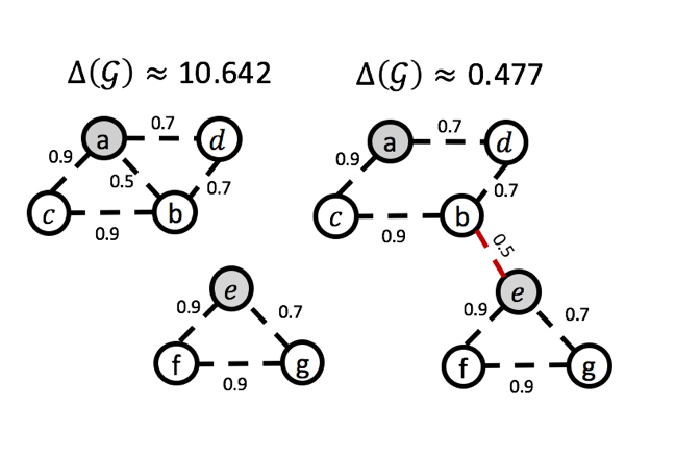
\includegraphics[scale=0.4]{figures/DegreeAUG/uncertainC.eps}
         \caption{\small{Resulting uncertain graphs}}
        \label{fig:edgeRelevance}
     \end{subfigure}
     \caption{Illustration of varying structural distortions by removing different uncertain edges $(b,e)$ and $(a,b)$ over an uncertain graph.}
     \label{fig:edgeRR}
\end{figure}
As exemplified in Figure~\ref{fig:edgeRR}, each edge modification will have \emph{varying} impact to the graph structure in the context of uncertain graphs. From the perspective of \emph{uniqueness}, nodes $a$ and $e$ are identical since adjacent edges have identical uncertainties. Accordingly, anonymity-oriented heuristics would select and perturb edges $(a,b)$ and $(b,e)$ without bias. As shown in Figure~\ref{fig:edgeRR}, the deletion of the uncertain edge $(b,e)$, the only link connecting two \emph{reliable} clusters, clearly incurs much larger structure distortion than the deletion of the edge $(a,b)$. This observation calls for an effective measure of edge influence in the context of uncertain graphs. 

Inspired by the significance of \emph{reliability}, we provide a compact analytic form of reliability deviation caused by individual uncertain edge modification in a fine-grained way, namely changing its edge probability in any granularity. Following the path, we introduce edge reliability relevance for edges' influence estimation, which can be quantified by the sum of reliability discrepancy of all the node pairs. Besides, we provide an algorithm for accessing edge \emph{reliability relevance} (RR) efficiently. 

\paragraph{Reliability Relevance Definition}

Lets start with analyzing the impact of single uncertain edge alteration to the connectivity of a specific node pair (Two-terminal Reliability).  
\begin{definition}
    \textbf{Two-terminal Reliability Relevance}
    Given an uncertain graph $\mathcal{G}$, and two nodes $u,v$, we consider the probability that $u$ is reachable to $v$,$R_{u,v}(\mathcal{G})$, as defined in Definition \ref{d:reliability}, as a multivariate function involving all the edge probabilities.   
    Thus, the partial derivative of $R_{u,v}(\mathcal{G})$ with respect to an individual variable $p(e)$, existence probability of an uncertain edge, denotes as $RR_{u,v}(e)$. It represents the sensitivity to the change of reliability $R_{u,v}$ which is determined by $p(e)$ with the others held constant. Its definitions is as follows:  
\begin{equation*}
    \svj
    RR_{u,v}(e)= \frac{\partial R_{u,v}(\mathcal{G})}{\partial \mathit{p}(e)}
    \svj
\end{equation*}
\end{definition}

% The following factorization lemma underlies the computation of partial derivative $RR_{u,v}(e)$ in a compact form. 
\begin{lemma}
    \textbf{Factorization Lemma}
       Given an uncertain graph $\mathcal{G}$, the reliability of the node pair $(u,v)$ $R_{u,v}(\mathcal{G})$ can factorized via one uncertain edge $e$ as follows:
    \vj
    \begin{equation*}
        R_{u,v}(\mathcal{G}) = p(e) R_{u,v} (\mathcal{G}_{e}) + (1-p(e)) R_{u,v} (\mathcal{G}_{\bar{e}} )
        \label{eq:fac}
        \svj
    \end{equation*}
    where uncertain graph $\mathcal{G}_{e}$ is identical with $\mathcal{G}$ except its edge $e$ is an \textbf{certain} edge. Similarly, the uncertain graph $\mathcal{G}_{\bar{e}}$ is identical with $\mathcal{G}$ except its edge $e$ is an \textbf{certain non} edge. 
\end{lemma}
According to the factorization lemma, the partial derivative $RR_{u,v}(e)$ can be rewritten as 
\vj
\begin{equation*}
    RR_{u,v}(e)=R_{u,v}(\mathcal{G}_{e})-R_{u,v}(\mathcal{G}_{\bar{e}})
\end{equation*}
\svj
The equation indicates the sensitivity of reliability is constant and it does not depend on the probability value of the uncertain edge $e$. Another important point to remember is that because all the connected pairs remain connected after the addition of an edge, $R_{u,v}(\mathcal{G}_{e}) - R_{u,v} (\mathcal{G}_{\bar{e}}) \ge 0$.

For a given uncertain edge $e$, the derivatives $RR_{u,v}(e)$ can be arranged in a $|V|\times |V|$ matrix, where each element corresponds to one node pair $(u,v)$ and it gives the partial derivative for the corresponding reliability $R_{u,v}$. As ever discussed, all the element are equal to or greater than zero.  
In this work, we define $RR(e)$ to be reliability relevance of an edge $e$ which can be quantified by the sum of all the $RR_{u,v}(e)$, as  
\vj
\begin{align*}
    RR(e) &= \sum_{u,v} |RR_{u,v}(e)| \\
          &= \sum_{u,v} |R_{u,v}(\mathcal{G}_{e}) -R_{u,v}(\mathcal{G}_{\bar{e}})| \\  
         &= \sum_{u,v} R_{u,v} (\mathcal{G}_{e}) - \sum_{u,v} R_{u,v}(\mathcal{G}_{\bar{e}})
    \svj 
\end{align*}
Note that, $RR(e)$ equals the difference of the expected number of connected pairs between uncertain graphs $\mathcal{G}_{e}$ and $\mathcal{G}_{\bar{e}}$ by explicit incorporation of edge uncertainty. In the context of edge relevance, reliability relevance can be seen as generalization of cut-edges, which quantifies the impact of partial edge deletion or addition on the connectivity in the uncertain graph. 
The higher reliability relevance score of an edge, the bigger impact of edge perturbation over the overall graph.  
On this basis, we define the reliability centrality of node $v$,$RC(v)$ to be the overall influence of graph reliability which can be quantified by the weighted sum of reliability relevance of all adjacent edges. 
\svj
\begin{equation*}
    RC(u)=\sum_{e} p(e) RR(e)
    \svj
\end{equation*}

\begin{algorithm}[!tb]
    \begin{algorithmic}[1]
       \item[] {\textbf{Input:} ~$\mathcal{G}=(V,E,\mathit{p})$, $K$ is the number of sampled graphs; usually $K=1000$}
    \item[] {\textbf{Output:} ~$RR$ Reliability relevance of edges in $\mathcal{G}$}
    \STATE {$CC_{e} \leftarrow  \mathbf{0} $, $CC_{\bar{e}} \leftarrow \mathbf{0}$}
    \FOR{i=1 \TO K }
    \STATE {$G \leftarrow $  A deterministic sampled instance}
    \STATE {$Ind(G)$ is edge existence of sampled graph $\mathcal{G}$}
    \STATE {$cc(G) \leftarrow $ the number of connected pairs of $G$}
    \STATE {$CC_{e}+=Ind(G) \cdot cc(G)$,$CC_{\bar{e}}+=(\mathbf{1}-Ind(G)) \cdot cc(G)$ }
    \ENDFOR
    \STATE{$RR= CC_{e}/\mathit{p} - CC_{\bar{e}}/{\mathbf{1}-\mathit{p}}$}
         \caption{Reliability Relevance Evaluation}
        \label{alg:RReval}
    \end{algorithmic}
\end{algorithm}


\paragraph{Reliability Relevance Evaluation}

Note that, the evaluation of $RR(e)$ need computing all the $R_{u,v}$ over two uncertain graphs $\mathcal{G}_{e}$ and $\mathcal{G}_{\bar{e}}$.  The two-terminal reliability detection problem is a $\#$P-complete problem \cite{MOBall}. Thus, the exact computation is not practical for large uncertain graphs. A basic approach is to get reliability approximation by sampling: for each uncertain edge $e$ 1) we first sample $K$ possible graphs $G_{1}, \ldots G_{K}$ of $\mathcal{G}_{\bar{e}}$ according to edge probability $\mathit{p}$, and 2) we then compute the number difference of connected pairs in each sample graph after edge $e$ is added. The basic sampling method can be rather computationally expensive. The total running time is $\Theta(|E| \cdot K\cdot \alpha(|V|) |E|)$ assuming incremental algorithm is used for computing connected components. It is impractical for large uncertain graphs with huge size of edges. 

Here, we introduce a much faster approach for computing $RR(e)$ as shown in Algorithm \ref{alg:RReval}. The basic idea is to partition all sampled graphs into groups according to existing edges so that the evaluation of the number of connected pairs can be reused. 
The complexity of reliability relevance evaluation of all edges is  $\Theta(K \cdot \alpha(|V|) |E|)$. 

\subsubsection{Reliability-oriented Edge Selection Procedure}

\input{Degree-AUG/genObfuscation.tex}
Now, we are ready to introduce our function \texttt{GenerateObfuscation} aims at finding a $(k,\epsilon)$-obf instance for an input \emph{uncertain graph} $\mathcal{G}$ using a given standard deviation parameter $\sigma$ as shown in Algorithm \ref{alg:genObf}. It resembles the method proposed in \cite{Boldi_Injecting_2012} with explicit incorporation of edge uncertainty in edge selecting and perturbing step. Another important contribution of our work is the utilization of reliability relevance (RR) for capturing structural relevance of edges in the uncertain graph.  

First, it computes the uniqueness level and reliability centrality for each node $v \in \mathcal{G}$. Intuitively, the more unique a node is, the harder it is to be obfuscated; the more \emph{important} an edge is, the bigger utility loss it incurs. Such heuristic information is important for our privacy-preserving and utility-preserving purpose. In order to  use the ``uncertainty budget'' in the most efficient way, the algorithm performs the following steps as shown in Algorithm \ref{alg:genObf}.

(Line 4: Excluding) Since it is allowed not to obfuscate $\epsilon|V|$ of the nodes, the algorithm selects the set $H$ of $\frac{\epsilon}{2}|V|$ nodes with largest uniqueness scores or reliability centrality scores, and exclude them from the subsequent obfuscation efforts. In later steps, the algorithm will inject uncertainty only to edges that are not adjacent to any of vertices in $H$. The key feature of our method is that it strictly preserve the 1-neighborhoods of influential nodes.  

(Line 8-18: Potential Edge Selection) The set of nodes not in $H$ will need to be anonymized. To anonymize more unique vertices, higher uncertainty is necessary. Thus, edges needed to be sampled with higher probability if they are adjacent to unique nodes. In order to better preserve graph structure, edges needed to be sampled with smaller probability if they are adjacent to more influential nodes. In order to handle this sample process, our algorithm assigns a probability $Q(v)$ to every $v \in V$, which depends on the uniqueness level $U(v)$ and reliability centrality $RC(v)$ of $v$. 

Each attempt begins by selecting a subset of edges $E_c$, which will be subjected to edge probability perturbation. Then set $E_{c}$, whose target size $\norm{E_c}=c \norm{E}$, is initialized to be $E$. Then, the algorithm randomly selects two distinct vertices $u$ and $v$, according to probability distribution $Q$. The pair of vertices $(u,v)$ is removed from $E_{c}$ with the probability $p(e)$ if it is an edge in the original graph, or added to $E_{c}$ otherwise.  The process is repeated until $E_{c}$ reaches the require size. In typical uncertain graphs, the number of non-edges is significantly larger than the number of uncertain edges, the loop ends very quickly, for small values of $c$. And, the resulting set $E_{c}$ includes most of edges in $E$. 

(Line 20) Next, we redistribute the perturbation budget among all selected edges $e \in E_{c}$ in proportion to their intermediate representations $Q(v)$. Specially, we define for each $e=(u,v) \in E_{c}$ , its uncertainty level, 
\vj
\begin{equation*}
Q(e):= \frac{Q(u)+Q(v)}{2}
\svj
\end{equation*}
and then set its edge perturbation parameter 
\vj
\begin{equation*}
\svj
\sigma(e)=\sigma |E_{c}|  \cdot \frac{Q(e)}{\sum_{e \in E_{c}} Q(e)}
\end{equation*}
so that the average of $\sigma(e)$ over all $e \in E_{C}$ equals $\sigma$.
\subsection{Anonymity-oriented Edge Perturbing}
\begin{figure}
    \captionsetup{justification=centering,margin=1cm}
       \begin{subfigure}[b]{0.45\textwidth}
        \centering
        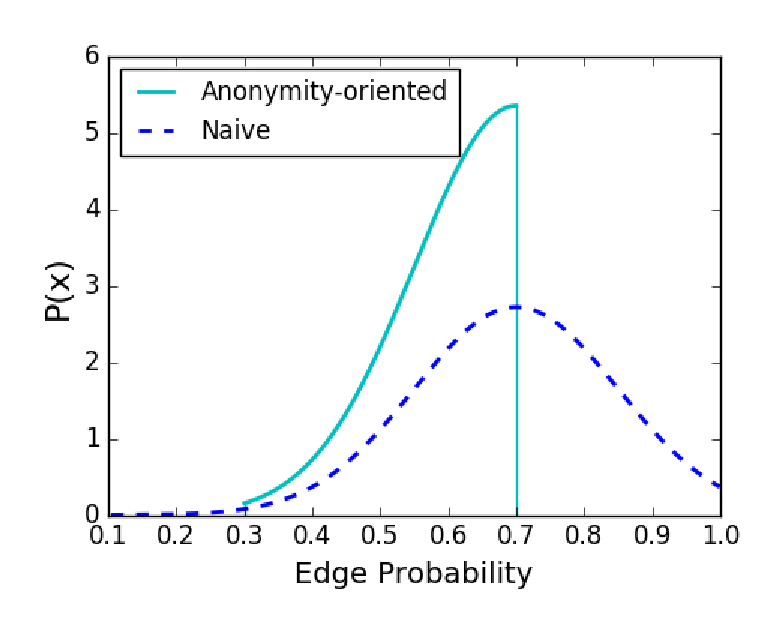
\includegraphics[scale=0.35]{figures/DegreeAUG/AnonymityEP.eps}
        \caption{\small{Anonymity-oriented Edge Perturbing}}
        \label{fig:anonymityEP}
    \end{subfigure}%
    \centering
        \begin{subfigure}[b]{0.45\textwidth}
            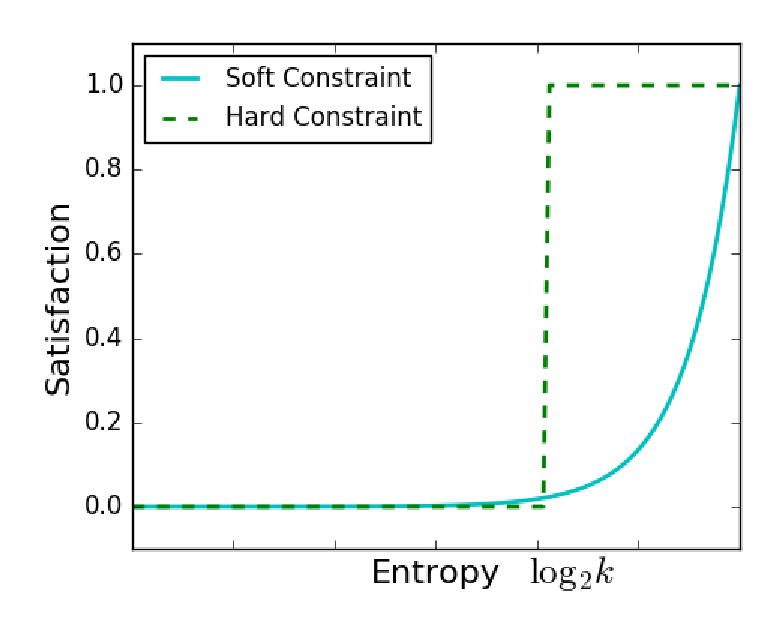
\includegraphics[scale=0.35]{figures/DegreeAUG/constraint.eps}
            \caption{\small{Relaxing $k$-obfuscation constraint}}
            \label{fig:constraintRelax}
        \end{subfigure} 
\end{figure}
As ever discussed, the existing uncertainty injecting scheme is designed for deterministic graphs and can not be used to handle uncertain graphs directly. Given the uncertainty level $\sigma(e)$, a natural strategy is to consider the partial edge addition and deletion in a random way as shown in Figure \ref{fig:anonymityEP}. Through the analysis of the impact of a single edge probability alteration, we give a anonymity-oriented perturbing heuristics which is able to constraint the potential range of edge prob perturbing (referred to C). For each selected edge $e \in E_{c}$ and the assigned uncertainty level $\sigma(e)$, we alter its existence probability as 
\vj
\begin{equation*}
    \tilde{\mathit{p}}(e):=\mathit{p}(e) + (1-2 \mathit{p}(e)) \cdot r_{e} 
    \svj
\end{equation*} 
Where the random perturbation $r_{e}$ is generated according to $\sigma(e)$ as Eq. \ref{eq:gen}. Namely, for an edge with the probability $p$, we only consider potential edge probability $\tilde{p}$ in the limited range that more likely contributes to higher graph anonymity. Clearly, previous scheme defined in deterministic graph becomes a special case of our approach. We proceed to elaborate the rationality and the benefit of this anonymity-oriented edge perturbing scheme by treating it as a constraint satisfaction problem. 
  
\subsubsection{Basics}
Let us consider $k$-obfuscate a given node $v$ as a single constraint $c_{v}$ for the target anonymization graph. Then, according to the definition \ref{obfCon}, the satisfaction of the constraint $c_{v}$ is defined as
\begin{equation*}
    \mathtt{c}_{v}:=
        \begin{cases}
                1  & H(Y_{P(v)}) \geq \log_{2}{k} \\
                0  & otherwise \\
         \end{cases}
\end{equation*}
Namely, given the considered degree-based re-identification scenario, we lower bound the entropy of degree distribution over the anonymized graph by $log_{2}{k}$. Accordingly, whether the anonymized graph $k$-obfuscates all the nodes can be expressed as degree of joint satisfaction.
\vj
\begin{align*}
    \mathcal{C(\mathcal{G})} &= \prod_{v \in V} \mathtt{c}_{v} \\
                &=\prod_{\omega} \underbrace{\mathtt{c} \ldots \mathtt{c}}_{s(\omega)}
    \svj
\end{align*}
The uncertain graph is said to $k$-obfuscate all the nodes if and only if the $C(\mathcal{G})$ equals 1.  
\subsubsection{Re-visiting graph anonymity}
As shown in Figure \ref{fig:constraintRelax}, the original satisfaction function is not everywhere differentiable.To simply the anonymity analysis, we approximate the individual constraint $c_{v}$ to a fuzzy relation in which the satisfaction degree of a constraint is defined as a continuous and differentiable function, going from fully violated to fully satisfied. A natural candidate for soft satisfaction function is,
\svj  
\begin{equation*}
    C_{v} = e^{H(Y_{P(v)})-\log_{2}{|V|}}
    \svj
\end{equation*}
According to this approximation, the satisfaction function of $k$-obfuscate all the nodes can be rewritten as
\svj
\begin{equation*}
   \mathcal{C}(\mathcal{G}) \propto \prod_{\omega} \underbrace{e^{H(Y(\omega)} \ldots e^{H(Y(\omega))}}_{s(\omega)}
\end{equation*}
While the original satisfaction is a binary value, the approximated satisfaction value lies in the continuous range $[0,1]$. Note that, the higher satisfaction score indicates the higher level of anonymity achieved. Taking logarithm for both side, we get the concise formula as 
\svj
\begin{equation*}
    \log \mathcal{C}(\mathcal{G})=\sum_{\omega} s(\omega) \cdot H(Y(\omega)
\end{equation*}
Regarding the property $P$, it equals the weighted sum of entropy over all possible values $\omega$, where $s(\omega)$ is the expected number of vertices with property value $\omega$ over all possible worlds. Targeting at high anonymity, we wish to increase the weighted sum of entropy. 

\subsubsection{Greedy search of graph anonymity}
% \begin{figure}
%     \centering
%     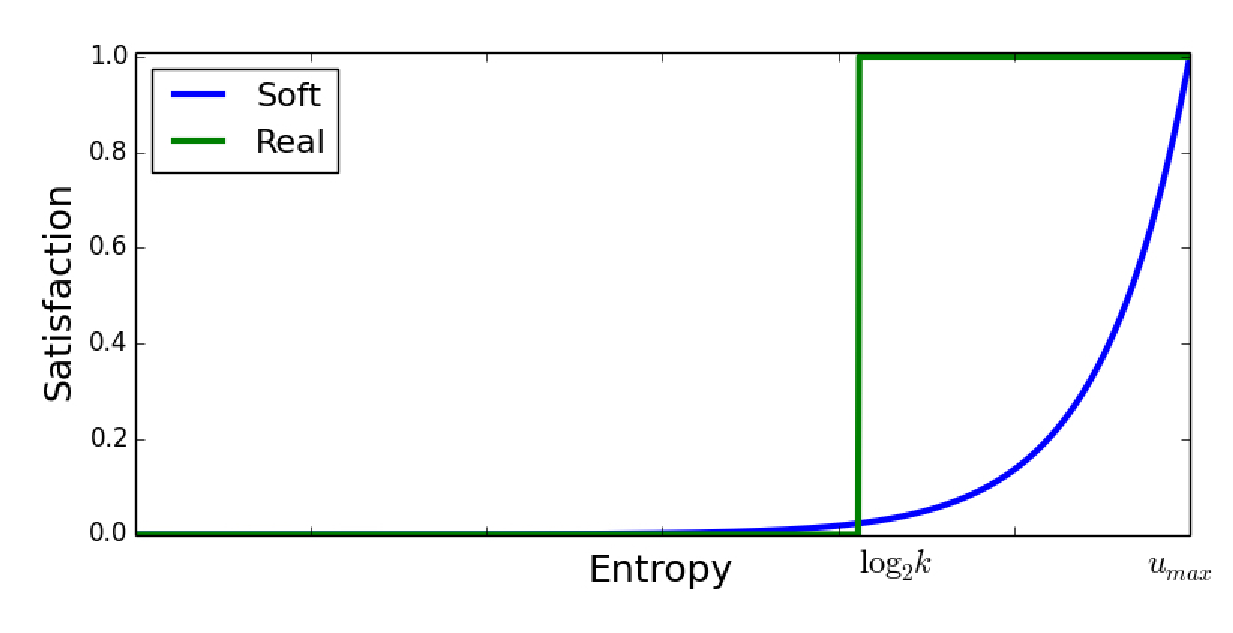
\includegraphics[scale=0.3]{figures/fuzzyConstraint.eps}
%     \caption{Relaxing Constraint}
%     \label{fig:rc}
% \end{figure}
The remaining issue is to connect the single edge probability alteration with the objective. With respects to node degree, a graph can be represented as one matrix as shown in figure \ref{fig:constraintRelax}. The weighted sum of entropy is related with graph coding. Here, we utilize entropy encoding, especially Huffman coding. From the coding perspective, we have two different angles to perform graph coding: row or column of degree matrix. The encoded length should be equal to each other, as shown in the following equation.  
\svj
\begin{equation*}
    \sum_{v} H(v) + n \log{n} = \sum_{\omega} s(\omega) \cdot H(Y(\omega))+ H(s(\omega))
    \svj
    \label{wegithedEn}
\end{equation*}
It indicates that higher global anonymity of a uncertain graph can be achieved by increasing the entropy of individual nodes when the global distribution $H(\omega)$ keeps constant. 

Note that, the probability change over a specific edge only affects degree distributions of its connected nodes. 
To further simply the problem, we assume that the impact of edge perturbing is independent to each other. Recall that, we suggest implementing perturbation to less anonymized nodes. In the case of degree obfuscation, they are nodes with high degree. For a node $v$ with high degree, the probability distribution of its degree $d_{v}$ may be approximated as the normal distribution as implied by the Central Limit Theorem. Hence, its induced entropy $H(v)$ can be approximated as $\frac{1}{2} {\ln (2 \pi e \sigma^2)}$. 

Targeting at maximizing the graph anonymity, we take steps proportion to the positive gradient with respect to the choice of individual edge probabilities. 
\svj
\begin{equation*}
    \frac{\partial \sum_{\omega} s(\omega) H(Y(\omega))} {\partial p(e)} \propto (1-2\mathit{p}(e))  
\end{equation*} 
Therefore, 
\vj
\begin{equation*}
    \tilde{\mathit{p}}(e):=\mathit{p}(e) + (1-2 \mathit{p}(e)) \cdot r_{e}
\end{equation*} 
Namely, our approach simulates one iteration of batch gradient ascent method for finding the local maximum of weighted entropy sum or the anonymity level. 
% \begin{algorithm}[t!]
	\begin{algorithmic}[1]
    	\item[] {\textbf{Input:}~Uncertain graph $\mathcal{G}=(V,E,\mathit{p})$, $ak,k,\epsilon,c,q$, \\and standard deviation $\sigma$ }
        \item[] {\textbf{Output:}~A pair $\langle \tilde{\epsilon}, \tilde{\mathcal{G}} \rangle$} 
        \STATE  {\textbf{compute} the uniqueness $U(v)$ for all the nodes}
        \STATE  {\textbf{compute} the \texttt{centrality} $RC(v)$ for all the nodes}
        \STATE  {$Q(v) \leftarrow U(v) \cdot RC(v)$}
        \STATE {$H \leftarrow$  the set of $\lceil \frac{\epsilon}{2} |V| \rceil$ with largest $Q(v)$}
        \COMMENT{Excluding}
     	\STATE {Normalized $RC(v)$; $Q(v) \leftarrow U(v) \cdot 1-RC(v)$;}
        \STATE {$\tilde{\epsilon} \leftarrow 1$}
   		\FOR{$t$ times} 
        	\STATE {$E_{C} \leftarrow E$} % either it become probabilistic 
            \COMMENT{Reliability-oriented Edge Selection}
         	\REPEAT  
            	\STATE{randomly pick a vertex $u \in V \setminus H$ according to $Q$}
            	\STATE{randomly pick a vertex $v \in V \setminus H$ according to $Q$}
            	\STATE{draw $w$ uniformly at random from $[0,1]$} 
            \IF {$(u,v) \in E$} 
				\IF {\texttt{$w > p(e)$}} 
                	\STATE {$E_{C} \leftarrow E_{c} \setminus \lbrace(u,v)\rbrace$}
                \ENDIF
            \ELSE \STATE{$E_{c} \leftarrow E_{c} \cup \lbrace(u,v)\rbrace$}
            \ENDIF 
            \UNTIL{$E_{C}=c|E|$}
            \FORALL {$e \in E_{C}$} 
            	\STATE {\textbf{compute} $\sigma(e)$}
                \COMMENT{Edge Probability Perturbation}
                \STATE {draw $w$ uniformly at random from $[0,1]$}
				\IF {$w < q$} \STATE{$r_{e} \leftarrow U(0,1)$}
                \ELSE 
                \STATE{$r_{e} \leftarrow R_{\sigma(e)}$}
                \ENDIF
                \STATE \textbf{$\tilde{p}(e) \leftarrow p(e)+ 2(0.5-p(e))\cdot r_{e}$}
            \ENDFOR
            \STATE {$\hat{\epsilon} \leftarrow checkAnonymity(\tilde{\mathcal{G}})$} 
            \COMMENT{Ensure Anonymity}
           	\STATE {Update result $\langle \tilde{\epsilon}, \tilde{\mathcal{G}} \rangle$ if $\hat{\epsilon}<\tilde{\epsilon}$}
        \ENDFOR 
        \STATE {return $\langle \tilde{\epsilon}, \tilde{\mathcal{G}} \rangle$}
      	\caption{GenerateObfuscation}
        \label{alg:genObf}
    \end{algorithmic}
\end{algorithm}



\chapter{Probabiltic Degree Anonymization over Uncertain Graphs}
\label{chp:e}
In this section, we formalize the threat of re-identification combined with the degree probability distributions in the context of uncertain graphs. We study the node degree information incoporates edge uncertainty and show its power to re-identify individual in a uncertain graph. Protecting against the threat of re-identification presents novel challenges for uncertain graph data. Generalization, random perturbation and uncertain graphs methods have been developed for determinitic graph anonymization. It is not trivial to shift these strategies for obfuscating degree probability distributions of nodes in the uncertain graph. 

% waiting for change 
% \section{Naive Approach: Anonymization via Representative Instance}
\label{sec:repOB}
\begin{figure}[t]
    \centering  
        \includegraphics[scale=0.38]{figures/DegreeAUG/repOB.eps}
    	\caption{Illustration of anonymizing an uncertain graph though its representative deterministic instance and its drawback.}
    \label{fig:repOB}
\end{figure}
A naive approach of anonymizing an uncertain graph is to first somehow transform it to a deterministic graph, then perform anonymization processing over the deterministic one. Fortunately, an increasing research effort was dedicated to the topic of exacting representative deterministic graphs from an uncertain graph \cite{Parchas_Gullo_Papadias_Bonchi_2014}. Parchas  {\etal} \cite{Parchas_Gullo_Papadias_Bonchi_2014} ever introduced algorithms for extracting deterministic representative graph which captures key properties of the input uncertain graph. Now, it becomes realizable to anonymize an uncertain graph in two steps as shown in Figure \ref{fig:repOB}. We first extract one deterministic representative instance $G$ from the input uncertain graph $\mathcal{G}$. Then, we anonymize the extracted deterministic graph $G$, and output this result as the anonymized result of the original uncertain graph $\mathcal{G}$ (referred as {\repAn}). 

The {\repAn} approach is attracting since it does not require any new anonymization techniques specific designed for uncertain graphs. When the extracted representative deterministic graph $G$ is close enough to the input uncertain graph $\mathcal{G}$ in terms of graph properties, its anonymized result is expected to be a good anonymization of the input uncertain one. However, there is a non-negotiable difference between the input uncertain graph $\mathcal{G}$ and its deterministic representative instance $G$, as exemplified in Figure \ref{fig:repOB}. The anonymized result of $G$ which is structurally similar to itself instead of the input uncertain graph, consequently, may be far different from the optimal solution, as exemplified in Figure \ref{fig:repOB}. Therefore, we believe that for many applications, the {\repAn} approach,  introducing a high level of noise in such fashion, do reduce the overall graph utility.  In experiment section, we will further illustrate this phenomenon over real-world datasets. 
\section{Probabilitic Degree-based De-anonymization}
In this section, we describe the threat of node re-identification in uncertain graph data, and we explain the content of external information and the use of external information in identifying anonymized individual. We develop the intuition behind achieving anonymity in an uncertain graph through structural similarity to others. 

Here, we remind the reader its difference compared to the deterministic case. The incorporation of uncertainty in the graph data significantly affects the distribution of vertex property. Existing graph perturbation techniques are not equipped to operate over uncertain graphs -- they will tend to ignore and destroy important structural properties. Likewise, uncertain graph structure and adversary knowledge with an incorporation of uncertainty to threaten privacy in new ways. 

\begin{figure}[t!]
    \centering 
    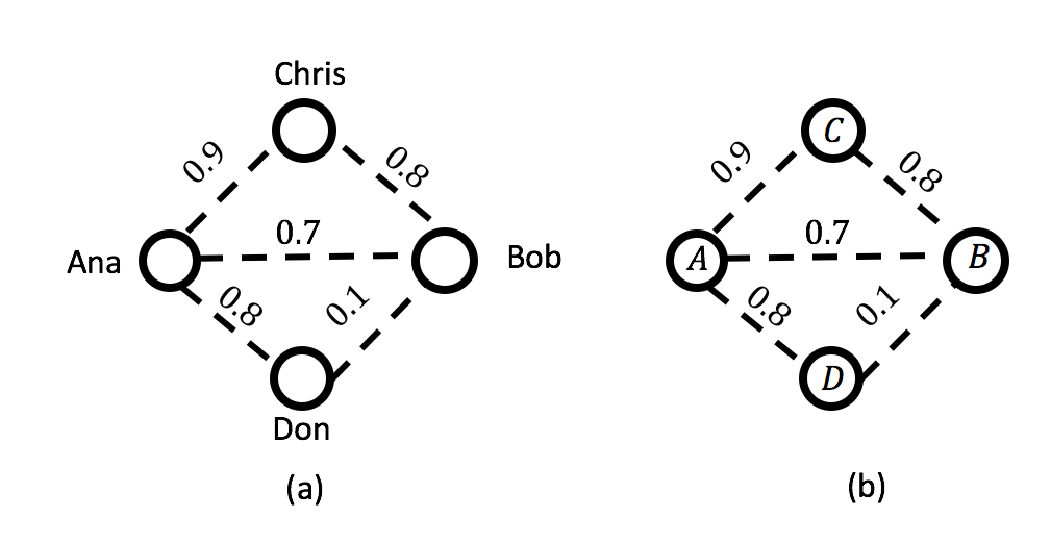
\includegraphics[scale=0.5]{figures/DegreeDistAUG/uncertainExample.eps}
    \caption{\small{(a) The original uncertain graph (b) The naive anonymized version of uncertain graph with 5 edges and $2^{5}=32$ possible world}}
    \label{fig:ddAUG:uncertainGraph}
\end{figure}

To gain more intuition on this attack model and the difficulties in defining a meaningful probabilistic matching, we present a simple example. Consider the original uncertain graph and the anonymized version of the given graph shown in Figure~\ref{fig:ddAUG:uncertainGraph}. We assume the adversary is equipped with the external structural information about some victim nodes. In particular, the property is node degree. Similarly, the degree of any nodes in the anonymized uncertain graph can be expressed as uncertain data. In the case of uncertain graph de-anonymization, the uncertainty belongs to the representation of source objects which are being identified, and the actual assertion is also probabilistic. In other words, fixed the node $v$ in the input uncertain graph, each node $u$ in the anonymized graph has a degree of being the image of $v$, which is probabilistic in nature. Meanwhile, the matching assertion is done by comparing two probability objects. 

\subsection{Adversary Knowledge}
We proceed to present the formal definition. Let us consider the knowledge that an adversary may extract from an uncertain graph about a given target vertex in $\mathcal{G}$. Following the literature, we assume that the adversary knows some vertex property $P$. In this work, we assume such property $P$ is the degree. Given an uncertain graph $\mathcal{G}$, each $v \in \mathcal{G}$ and the degree value $\omega$, we define the probability that $X_{v}(\omega)$ that $v$ originated from a vertex in $G$ with property value $\omega$. Specifically, 
\begin{equation*}
    X_{v}(\omega) = \sum_{G \in W(\mathcal{G})}  Pr(G) \cdot \mathcal{X}_{v,\omega}(G)
\end{equation*}
where $Pr(G)$ is the probability that the possible world $G$ is observed, and $\mathcal{X}_{v,w}(G)$ is 0-1 variable that indicates the vertex $v$ has the degree value $\omega$ in the possible world $G$. In other world, $X_{v}(\omega)$ is the sum of probabilites of all possibel worlds in which the vertex $v$ has the given property value $\omega$. We define the degree value of a node $v$ in an uncertain graph $d_{v}$ as an random variable with a probability distribution $X_{v}$. The probabilties $X_{v}(\omega)$ may be arrange in a $n \times |\Omega|$ matrix, where each row corresponding to one vertex $v in \mathcal{G}$ and it gives the probability distribution $X_{v}$. 
 \begin{table}[t!]
     \centering
      \begin{tabular}{|L{1.25cm}|c|c|c|c|}
             \cline{1-5}
                $\mathbf{X}_{v}(\omega)$ & $\text{deg}=0$ & $\text{deg}=1$ & $\text{deg}=2$ & $\text{deg}=3$ \\ \hline 
              $a$   & $0.006$ & $0.092$ & $0.398$ & $0.504$ \\ 
              $b$   & $0.054$ & $0.348$ & $0.542$ & $0.056$  \\
              $c$   & $0.020$ & $0.260$ & $0.720$ & $0.000$ \\
              $d$   & $0.180$ & $0.740$ & $0.080$ & $0.000$  \\  \hline 
 %              $\mathbf{S(\omega)}$   & $0.260$ & $1.440$ & $1.740$ & $0.560$ \\ \hline 
      \end{tabular} 
      \caption{The matrix $X_{v}(\omega)$ for the uncertain graph in Figure~\ref{fig:ddAUG:uncertainGraph} and the degree property.}
     \label{tab:DegreeMatrix}
 \end{table}


\begin{example}
    Consider the uncertain graph in Figure~\ref{fig:ddAUG:uncertainGraph} and assume the vertex property is degree. Table \ref{tab:DegreeMatrix} gives the corrsponding matrix $X_{v}(\omega)$, in which each row gives the probability distribution regrading the dgree of the corresponding vertex in $\mathcal{G}$. For instance, the probability that $a$ has degree $3$ is $0.9 \cdot 0.7 \cdot 0.8=0.504$. 
\end{example}

\subsection{Re-identification Attack}
The degree value of a node $u$ in the anonymized uncertain graph is defined as the corresponding random variable $d_{u}$.  The matching assertion is evaluated as the probability of the event two random variable $d_{u}$ and $d_{v}$ is equal. Specifically, 
\begin{align*}
    F_{u}(v)=P(d_{u}=d_{v})&=\sum_{\omega} P(d_{u}=\omega) \cdot P(d_{u}=\omega) \\
                  &=\sum_{\omega} X_{v}(\omega) \cdot X_{u}(\omega)
\end{align*}
The probabilities $F_{u}^{v}$ may be arrange in a $n \times n$ matrix, where each row corresponds to one vertex $u \in \tilde{\mathcal{G}}$ and it gives the corresponding probability $F_{u}^{v}$ over all possible target nodes $v \in V_{\mathcal{G}}$. The columns of that matrix are proportional to the probability distribution that correponding to victim nodes. More precisely, the normalized column corresponding to a target node $v$, {\ie}, 
\begin{equation*}
    Y_{v}(u):=\frac{F_{u}(v)}{\sum_{u \in \tilde{G}} F_{u}^{v}}
\end{equation*}
is the probability that $u$ is the image in $\tilde{\mathcal{G}}$ of a vertex that had property $d_{v}$ in $\mathcal{G}$.

 \begin{table}[t!]
     \centering
    \begin{tabular}{|L{1.25cm}|c|c|c|c|}
      \cline{1-5}
      $\mathbf{F_{u}^{v}}}$ & $v_{a}$ & $v_{b}$  & $v_{c}$ & $v_{d}$ \\ \hline 
      $u_{a}$ & 0.42092 & 0.27628 & 0.3106  &  0.101 \\
      $u_{b}$ & 0.27628 & 0.42092 & 0.4818 &  0.3106 \\
      $u_{c}$ & 0.3106  & 0.4818  & 0.5864 &  0.2536 \\
      $u_{d}$ & 0.101   & 0.3106  & 0.2536 &  0.5864 \\  \hline 
    \end{tabular}
    \caption{The matrix $F_{u}^{v}$ for the uncertain graph and itself in Figure~\ref{fig:ddAUG:uncertainGraph} and the degree property.}
    \label{tab:DegreeDistMatching}
 \end{table}


 \begin{table}[t!]
     \centering
    \begin{tabular}{|L{1.25cm}|c|c|c|c|}
      \cline{1-5}
      $\mathbf{Y_{u}^{v}}}$ & $v_{a}$ & $v_{b}$  & $v_{c}$ & $v_{d}$ \\ \hline 
      $u_{a}$ & 0.37962     & 0.18548  & 0.19027  &  0.08069 \\
      $u_{b}$ & 0.24917     & 0.28257  & 0.29515  &  0.24816 \\
      $u_{c}$ & 0.28012     & 0.32344  & 0.35922  &  0.20262 \\
      $u_{d}$ & 0.09109     & 0.20851  & 0.15535  &  0.46852 \\  \hline 
    \end{tabular}
    \caption{The matrix $Y_{u}^{v}$ for the uncertain graph and itself in Figure~\ref{fig:ddAUG:uncertainGraph} and the degree property.}
    \label{tab:DegreeDistPreimage}
 \end{table}

\begin{example}
    For example, if in the anonymization process we do nothing, then the perturbed output $\tilde{\mathcal{G}}=1$. In the case, the probability matrix induced by $\tilde{\mathcal{G}}$ equals to the one induced by $\mathcal{G}$. Table \ref{tab:DegreeDistMatching} gives the corresponding matrix $F$. For instance, the probability that $d_{a}$ is equal to $d_{c}$ is $0.006 \cdot 0.02 + 0.092 \cdot 0.26 + 0.398 \cdot 0.72 + 0.504 \cdot 0=0.3106$. After normalization them, give the corresponding $Y_{u}(v)$  distributions for each vertex $v$ in Table \ref{tab:DegreeDistPreimage}. For instance, if we look for a vertex that has the same degree distribution of $Ana$ in $\mathcal{G}$, it is either $a$, with probability around $0.38$, $b$ with probability around $0.25$, $c$ with probability around $0.28$, or $d$ with probability around $0.09$. 
\end{example}

\subsection{Privacy Notation}
Likewise, we can define our notion of privacy . 
\begin{definition}
    \textbf{\boldmath{$(k,\epsilon)$}-obf \cite{Bonchi_Identity_2014}}
    Let $P$ be the degree distribution, $k \geq 1$ be a desired level of anonymity, and $\epsilon >0 $ be a tolerance parameter. The uncertain graph $\tilde{\mathcal{G}}$ is said to $k$-obfuscate a given vertex $v \in V_{\mathcal{G}}$ with respect to $P$ if the entropy of the distribution $Y_{v}$ over the vertices of $\mathcal{G}$ is greater than or equals to $\log_{2}{k}$:
    \vj
    \begin{equation*}
        H(Y_{v}) \geq \log_{2}{k}.
    \label{obfCon}
    \svj
    \end{equation*}
The uncertain graph $\mathcal{G}$ is $(k,\epsilon)$-obf with respect to property $P$ if it $k$-obfuscates at least $(1-\epsilon)|V|$ vertices in $V_{\mathcal{G}}$. $P$ can be any node properties.  
\end{definition}
Namely, given the considered attack scenario, in which the adversary uses the degree distribution information of his target vertex $v$, we wish to lower bound the entropy of the distribution it induced over the perturbed graph vertices by $\log_{2}{k}$. The general idea is exact the same with {\keobf}, proposed in the literture~\cite{Bonchi_Identity_2014}. We extend the concept of equivalent class to probabilitic scenerio. 
\section{Probabilitic Degree Anonymization}
The uncertainty injecting scheme resembles the degree anonymization method designed for the deterministic graph. One common heuristics is to select the perturbation budget for each selected edge $e=(u,v)$, depending on properties of  the vertices $u$ and $v$. The perturbation will be larger for edges that connect unique vertices, which, require higher levels of uncertainty to ``blend in the crowd", and smaller for edges that connect more ``typical" vertices. Note that, it requires one effective method to capture how typical a given vertex is among all the vertices in the uncertain graph, in terms of vertex property $P$. In this work, let us consider vertex property $P$ be node degree. In this case, namely, it is related to cluster uncertain data (distribution). The key feature of our method is to incorporate the statistical distance function for calculating the uniqueness level of vertices with regards to their node degree. 

\subsection{Uniqueness Score of Vertices}
\begin{figure*}[t!]
     \begin{subfigure}[b]{1\textwidth}
        \centering
        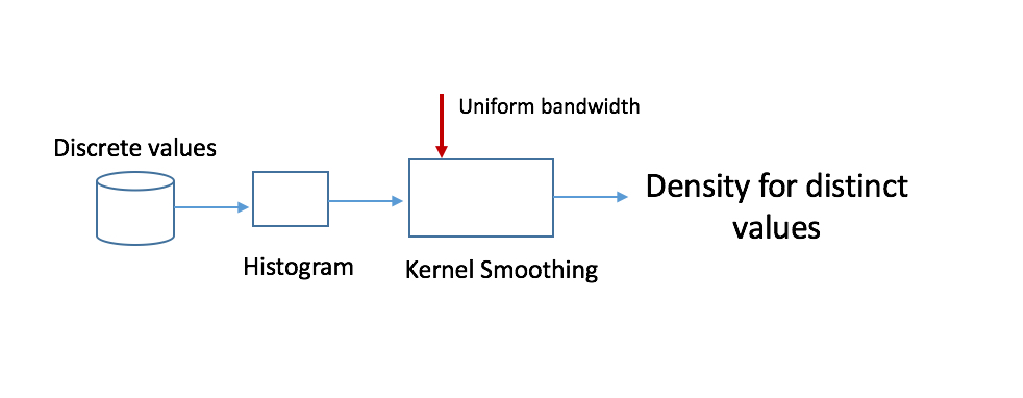
\includegraphics[scale=0.7]{figures/DegreeDistAUG/uniqueD.eps}
        \caption{Density estimation of nodes degree (Determinitic cases)}}
        \label{fig:uniqueDcal}
    \end{subfigure}%
    \begin{subfigure}[b]{1\textwidth}
		\centering
        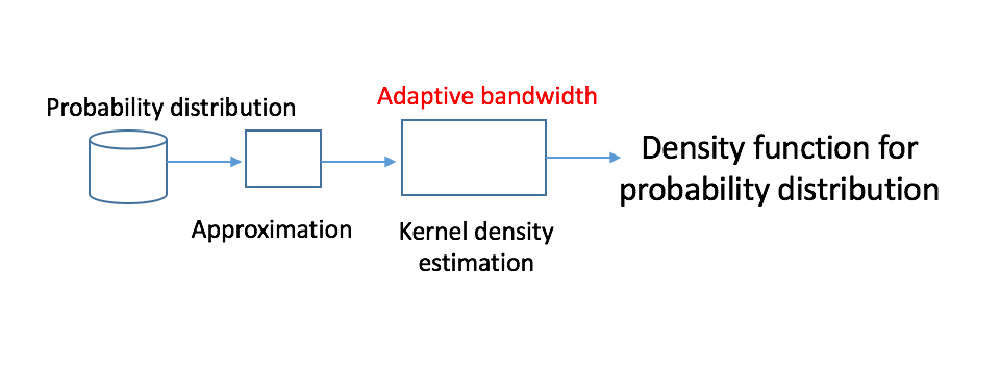
\includegraphics[scale=0.7]{figures/DegreeDistAUG/uniqueDD.eps}
        \caption{Density estimation of nodes degree (Uncertain cases)}}
        \label{fig:uniqueDDcal}
    \end{subfigure} 
    \caption{Comparison of determinitic and uncertain vertex density estimation in terms of node degree.}
\end{figure*}
For vertex properties of interest, such as degree, the majority of vertices in the real uncertain graphs are already anonymous even without random perturbation. The phenomena inherit from the one in the deterministic graph. The majority of vertices in the graph have a low degree ($\le 10$) with quite similar distribution. Hence, we aim at controlling the amount of applied perturbation, so that larger perturbation is added at vertices that are less anonymized in the original graph, namely, outlier point with respects to its degree distribution. In particular, we suggest calibrating the perturbation applied to an edge $e=(u,v) \in E_{c}$ according to the ``uniqueness" of the two vertices $u$ and $v$ with respect to the property $P$. Namely, if both $P(u)$ and $P(v)$ are in the dense region, then $r_{e}$ should be very small; on the other hand, if $P(u)$ and $P(v)$ are outlier values, then $r_{e}$ should be higher. The definition is quite similar to the ``uniqueness score", proposed in~\cite{} while extended for dealing with uncertain objects. 

Let $P$: $V \rightarrow \Omega$ be node degree defined on the set of vertices $V$ in an uncertain graph. Clearly, $\omega$ denotes uncertain object (random variable). Further, consider a distance function $d$ between  random variables in the range $\Omega$. So, for each pair of random variables,$p$ and $q$, distance $d(p,q) \ge 0$ is defined. For the degree property $P_{1}$, a natural candidate of statistical distance function is Bhattacharyya distance. For probability distribution $p$ and $q$ over the same domain $X$, the Bhattacharyya distance is defined as: 
\begin{equation*}
    D_{B}(p,q)=-ln(\sum_{x} \sqrt{p(x) \cdot q(x)})
\end{equation*}
Before the computing of statistical distance between probability distributions, we need to get the probability distribution for all the vertices in the uncertain graph. The probability distribution of $d_{v}$ may be computed exactly in time $O(n^2)$ or be approximated in time $O(n)$. The statistical distance between two probability distribution may be computed exactly in time $O(n)$. The overall complexity is $O(n^{3})$. Clearly, it is not suitable for large uncertain graphs. Note that, the uniqueness function is used for locating outlier points. For the degree property, they are nodes with high degree. In such case, we may adopt an alternative approach. Since the $d_{v}$ is the sum of independent random variable, it may be approximated by the normal distribution $N(\mu, \sigma^{2})$, where $\mu= \sum p_{e_i}$  and $\sigma^2= \sum p_{e_i} \cdot (1-p_{e_{i}})$ as implied by the Central Limit Theorem. The Central Limit Theorem becomes effective already for $n \approx 30$. For typicals size of $n$ in large uncertain graphs, the normal approximation becomes very accurate. According to the normal approximation, the Bhattacharyya distance between two normal distribution can be cacluated~\cite{} by exacting the mean and variances of two separate distribution objects: 
\begin{equation*}
    D_{B}(p,q)=\frac{1}{4} \cdot \ln{\frac{1}{4} 
                (\frac{\sigma_{p}^2}{\sigma_{q}^2} + \frac{\sigma_{q}^2}{\sigma_{p}^2}+2)}+
                \frac{1}{4} \cdot (\frac{(\mu_{p}-\mu_{q})^{2}}{\sigma_{p}^2+ \sigma_{q}^2})
\end{equation*} 
By this way, we map the object (probability distribution) from high dimension to 2D space. It speed up the computation of ``uniqueness score''. The overall time complexity is $O(n^2)$ where $n$ is the number of vertices in the uncertain graph. The quartic complexity is not suitable for dealing with large networks. 

Note that, the definition of the uniquness score is related to the kernel density estimation. For the specific method proposed in the literture~\cite{Boldi_Injecting_2012}, it adopts the gaussian function as a weighting function (kernel), the absolute difference as a distance function and the parameter $\theta$ for setting bandwidth. H
For computing the distance between probability distributions, the statistical distance functions were choosed. The remaining issue is the choice of bandwidth. Note that, the choice of bandwidth has the siginificant effect on the shape of the corresponding kernel density estimator. If the bandwidth is small, we will obtain an under smoothed estimator, with high variability. On the contrary, if the value of bandwidth $h$ is big, the resulting estimator will be over smooth and farther from the real data distribution that we are trying to estimate. Notice of the connection between uniqueness and density estimation, we adopt the adaptive bandwidth kernel density estimation method, {\ie}, we vary the w of the kernel in different regions of the sample space. By this way, we can get the statistical robust estimation of the distribution of all the vertices in the input uncertain graph in an efficient way. 

\subsection{Proposed Research Tasks}
\begin{itemize}
    \item {We identify and formulate the node re-identification attack using their degree probability distribution, and extend the {\keobf} notation for quantifying privacy level. We present the reliability and privacy preserving problem in the context of uncertain graphs.}
    \item {We show case that a naive approach that simply combines existing techniques do not work in practice due to significant utility loss.}
    \item {We propose a heuristic based on the density estimation of probability distributions among all the vertices in the uncertain graph for injecting perturbation judiciously. We give an efficient and effective method for heuristic evaluation.}
    \item {We propose to explore different search strategy for solving the induced optimized problem in the process of injecting uncertainty. }
    \item {We perform an extensive experimental evaluation using four real-world uncertain graph data sets from different  domains. We evaluate and compare our methods using different groups of graph metrics.}
\end{itemize}
\clearpage
\chapter{Research Schedule}
\label{chp:schedule}
It is planned to finish the dissertation work by May 2017. The tentative research schedule is listed as follows. Note that the schedule is made based on current progress. 

\bigskip

\begin{tabular}{|l|p{.59\textwidth}|}
%\begin{tabular}{|l|l|}
\hline Time & Tasks \\ \hline
Now - March 2017 &  Degree Distribution Anonymization on Uncertain graphs: Explore the uncertain graph mofiication techniques for anonymizing degree distribution; Explore the randomized strategy for justificious uncertain graph modifiaction; Implement our proposed techniques; Conduct performance evaluation; Write paper
\\ \hline
March 2017 - May 2017 &  Dissertation writing
\\ \hline
May 2017 & Dissertation defense\\ \hline
\end{tabular}

\bigskip

I plan to write the following paper.
\begin{itemize}
\item ``Degree Distribution Anonymization on Uncertain Graphs'' to VLDB 2017
\end{itemize}

\bibliographystyle{abbrv}
\bibliography{bermuda.bib,aug.bib}
\end{document}

